\documentclass[12pt]{article}

\usepackage{amssymb,amsmath,amsfonts,booktabs,eurosym,geometry,ulem,graphicx,caption,color,setspace,sectsty,comment,float,footmisc,caption,natbib,pdflscape,pdfpages,array,hyperref,amsmath,subcaption}

\normalem

\onehalfspacing
\newtheorem{theorem}{Theorem}
\newtheorem{corollary}[theorem]{Corollary}
\newtheorem{proposition}{Proposition}
\newenvironment{proof}[1][Proof]{\noindent\textbf{#1.} }{\ \rule{0.5em}{0.5em}}

\newtheorem{hyp}{Hypothesis}
\newtheorem{subhyp}{Hypothesis}[hyp]
\renewcommand{\thesubhyp}{\thehyp\alph{subhyp}}

\newcommand{\red}[1]{{\color{red} #1}}
\newcommand{\blue}[1]{{\color{blue} #1}}

\newcolumntype{L}[1]{>{\raggedright\let\newline\\arraybackslash\hspace{0pt}}m{#1}}
\newcolumntype{C}[1]{>{\centering\let\newline\\arraybackslash\hspace{0pt}}m{#1}}
\newcolumntype{R}[1]{>{\raggedleft\let\newline\\arraybackslash\hspace{0pt}}m{#1}}

\geometry{left=1.0in,right=1.0in,top=1.0in,bottom=1.0in}

\begin{document}

\begin{titlepage}
  \centering
  
\includegraphics[height=4cm]{UoB_RGB_24.jpg}\par\vspace{0.5cm}
  \vspace{2 cm}

  % Dissertation title
  \hrule height 0.4pt
  \vspace{1cm}
  {\bfseries\large How Internal Immigration Drives Knowledge Inflow: Insights from China's Patent Citations\par}
  \vspace{1cm}
  \hrule height 0.4pt
  \vspace{4cm}

  % Student details
    \textbf{
    Student number: 2523377 \\
    Word count: 14877      \\
    Date submitted: \today \\
    Programme: MSc Economics}

  \vspace{4cm}
  % Declaration
  \begin{minipage}{0.82\textwidth}
    \footnotesize
    \emph{“A dissertation submitted to the University of Bristol in accordance with the
    requirements of the degree of Master of Economics in the Faculty
    of Social Sciences and Law.”}
  \end{minipage}\par\vfill

  % Footer line
  \begin{tabular*}{\textwidth}{@{}l@{\extracolsep{\fill}}r@{}}
    School of Economics & August 2025
  \end{tabular*}
  \setcounter{page}{0}
  \thispagestyle{empty}
  \clearpage
\end{titlepage}

\begin{abstract}
\noindent 
This dissertation examines whether internal migration facilitates the diffusion of technological knowledge across Chinese cities. I assemble a city--year panel for 2010--2016 that links migrant stocks by origin province from the China Migrants Dynamic Survey to directional patent backward citations from the China National Intellectual Property Administration. To address endogeneity of migrantion, I use a leave-out shift--share instrument that interacts cities' baseline migrant origin-shares with origin-specific outmigration shocks, and construct migrant fractions using a predicted-population denominator.

The IV estimates indicate that migrant inflows are associated with higher knowledge inflows: a 1\% increase in a city's migrant share corresponds to about a 0.65\% increase in backward citations. High-skilled migrants have a five times larger effect than baseline. While effect for recent arrivals is insignificant. Migration is more closely linked to invention patent citations than to utility. Estimates are small on the eastern while larger in central and western cities. Immigrants can facilitate both indirect or direct knowledge inflow

The study contributes (i) evidence on the innovation consequences of internal migration, (ii) a city-level, directional measure of within-country knowledge flows based on patent citations in China, and (iii) an assessment of heterogeneity by migrant composition, patent type, and region. The findings suggest that policies easing internal mobility can support the diffusion of knowledge.
\\
\vspace{0in}\\
\noindent\textbf{Keywords:} Internal migration; Knowledge diffusion; Patent citations; Innovation spillovers; Shift-share instrument; China; Hukou reform\\
\vspace{0in}\\
\noindent\textbf{JEL Codes:} J61, O31, O33, R23, R11\\
\vspace{0in}\\
\bigskip
\setcounter{page}{0}
\thispagestyle{empty}
\clearpage
\end{abstract}

\section*{} %dedication and knowledgement
\noindent \textit{This dissertation is dedicated to my family, whose unwavering support have been the cornerstone of my academic journey. Their belief in me has provided continuous motivation, inspiring me to pursue my goals and strive for excellence.\\
I am also deeply grateful to my supervisor, Davide M. Coluccia, for his steadfast guidance and support throughout this project. I feel truly fortunate to have been his student—from attending his Labour Economics lectures to working under his supervision on this dissertation. His mentorship has been invaluable to both my studies and personal growth.\\
And last but not least, I would like to thank the University of Bristol for providing a stimulating academic environment and the resources that made this research possible.}
\setcounter{page}{0}
\thispagestyle{empty}
\clearpage

\section*{Declaration}
\noindent
I declare that the work in this dissertation was carried out in accordance with the requirements of the University's Regulations and Code of Practice for Taught Programmes and that it has not been submitted for any other academic award. Except where indicated by specific reference in the text, this work is my own work. Work done in collaboration with, or with the assistance of others, is indicated as such. I have identified all material in this dissertation which is not my own work through appropriate referencing and acknowledgement. Where I have quoted or otherwise incorporated material which is the work of others, I have included the source in the references. Any views expressed in the dissertation, other than referenced material, are those of the author.

\vspace{1.5cm}

SIGNED: \\

DATE: \today
\setcounter{page}{0}
\thispagestyle{empty}
\clearpage


\renewcommand{\contentsname}{Table of Contents}
\tableofcontents
\setcounter{page}{0}
\thispagestyle{empty}
\clearpage

\pagebreak \newpage
\doublespacing


\section{Introduction} \label{sec:introduction}

Knowledge diffusion --- the spread of ideas, technologies, and expertise --- is a fundamental driver of innovation and long-run economic growth. One important mechanism facilitating such diffusion is migration, through which individuals carry knowledge and skills across regions and establish networks that transmit information. A rich body of research has documented the role of international migration in transferring knowledge across borders and boosting innovation in destination economies. For example, studies find that immigrants can increase patenting and productivity in host countries by bringing diverse expertise and connections (e.g. \cite{kerrEthnicScientificCommunities2008, baharMigrationKnowledgeDiffusion2018, lissoniMigrationInnovationLearning2024}). In contrast, the contribution of internal (within-country) migration to knowledge diffusion remains comparatively less explored. This gap is particularly notable in the case of China, a country with massive internal migrant flows and a unique household registration (hukou) system that historically constrained mobility. Only recently have a few studies begun to examine internal migration's impact on innovation in China: for instance, \cite{guanHowDoesLargescale2025} show that greater migrant inflows causally increased cities' patent outputs (especially via high-skilled migrants), and \cite{gaoSpatialSpilloverEffects2024} report that inter-provincial migration of skilled workers yields positive innovation spillovers. However, these works use aggregate innovation measures and leave open questions about the specific knowledge transmission channels and the extent of causality. This dissertation addresses these gaps by investigating whether and how internal migration contributes to the within-country diffusion of knowledge in China's fast-evolving economy.

The study examines the impact of internal migration on knowledge inflows into Chinese cities, leveraging patent citations. China's context offers an ideal setting for this inquiry --- the country has experienced rapid economic transformation alongside large-scale internal migration, under institutional constraints like the hukou system that make migration patterns selective. Focusing on patent citations as a measure of knowledge flow allows for a direct observation of innovation spillovers: when a new patent in a city cites prior art from elsewhere, it provides tangible evidence of knowledge being transmitted to that city. By linking migrants to these citation flows, I can trace how ideas from migrants' origin locations propagate to their destination cities. In contrast to prior studies that rely on broad innovation indicators (e.g. total patent counts or R\&D spending), this approach pinpoints directional knowledge transfer and thus sheds light on the mechanisms of diffusion. Specifically, the analysis matches city-level migrant stocks by origin province with the network of patent backward citations (references to earlier patents) to test whether migrant inflows facilitate new ideas flowing from the migrants' home regions to the destination citise. By examining this relationship in the setting of China's internal migration, the study provides evidence from an emerging economy context that has received limited attention in the knowledge diffusion literature.

Estimating the causal effect of migration on knowledge diffusion is challenging because of migrantion is not random. Migrants might be drawn to cities that are already innovative, or other unobserved factors like policy changes could drive both migration and knowledge production. To address this concerns, the study employs a shift-share instrumental variable (SSIV) strategy. The intuition is to isolate variation in migration flows that is exogenous to local innovation shocks. In practice, the instrument is constructed by interacting historical migration patterns with external shocks to migration. First, each city's baseline distribution of migrants by origin (e.g. the provinces that historically sent migrants to that city) is measured. This captures the “share” component --- the pre-existing migrant network ties. Second, I use plausibly external “shifts” in migration push factors affecting those origin provinces (for example, policy changes, economic downturns, or natural shocks that increase out-migration from certain provinces). By multiplying the city's historical origin-share by the time-varying origin shock, I predict the inflow of migrants to the city that is driven by conditions in the migrants' home provinces rather than by the destination city's current characteristics. This SSIV generates quasi-experimental variation in internal migration: effectively, some cities receive more migrants due to push forces outside the city, not because the city itself became more attractive for innovation. This helps to mitigate endogeneity, ensuring that I am able to measure the causal impact of migrant inflows on knowledge outcomes. 

Beyond the overall impact, the dissertation delves into which migrants and where have the strongest knowledge diffusion effects. First, it estimate the effect of high-skilled migrants, as well as recent migrants, in driving knowledge inflows. This allows me to identify which groups of migrants contribute the most to spreading innovation --- for instance, whether cities benefit more from an influx of educated professionals versus unskilled labour, and whether migrants begin contributing immediately or only after assimilating for some years. Second, the study examines regional heterogeneity. China's cities vary widely in development; the analysis tests whether migrant-induced knowledge spillovers are more pronounced in less-developed inland regions compared to the advanced eastern coastal region. This geographic lens is important for understanding if migration helps reduce regional innovation disparities or if its benefits concentrate in already-developed hubs. Third, the research differentiates between types of knowledge diffustion by analyzing patent sub-categories. By comparing the effects of migration on citations in invention patents versus utility models, the study pinpoints whether migration primarily fosters frontier, novel innovation or more modest, incremental knowledge diffusion. By distinguishing external citations from self-citations,the study also examines whether immigrants bring knowledge directly or indireclty.

The empirical findings demonstrate that internal migration indeed serves as an important channel of knowledge diffusion within China. In summary, cities that attract more migrants experience greater inflows of external patent knowledge. The Ordinary Least Squares (OLS) estimates a 1.148\% increase. Importantly, after accounting for endogeneity via the IV approach, the estimates remains is more modest in magnitude. This suggests that part of the naive association was inflated by selective migration --- i.e. more innovative cities tend to attract more migrants. Even so, the Two-Stage Least Squares (2SLS) results confirm a causal knowledge spillover effect: an increase in migrant inflows leads to a 0.65\% increase in knowledge inflow. Turning to heterogeneity, the composition of migrants is crucial. 
High-skilled migrants emerge as key vectors with a 3.245\% increase on knowledge inflows which is around five times larger than general migrants. By contrast, recent migrants (those who arrived within 1 year) do not show an significant effect. This may imply that migrants contribute to innovation after gaining some local experience or that there is a lag before their knowledge is effectively absorbed by the host city. 
In terms of types of patent, migrant inflows have a effect on invention patents with 0.646\% increase while no significant effect on utility patents.
Consistently, migration-driven citations occur both through external citations and self-citations, with 0.639\% and 0.764\% increases respectively. 
Finally, there is notable regional variation: the knowledge spillover benefits of migration are disproportionately high for China's mid-western and inland regions compared to the eastern coast. 
Collectively, these results paint a comprehensive picture of internal migration as a driver of domestic knowledge diffusion, while also delineating the conditions and channels through which its impact is realized.

This research makes several contributions to the literature. First, it adds to the broad migration and development literature by focusing on internal migration and demonstrating its impact on innovation within a developing country context. Prior migration studies on China have largely centered on labour market and productivity effects or treated migration as a reallocative force; this work shifts the focus to migrants' role as carriers of knowledge, thereby extending our understanding of migration's economic consequences beyond labour or demographic outcomes. Second, the study contributes to the knowledge diffusion literature, particularly research using patent data, by utilizing patent citation networks to trace knowledge flows inside a country. This offers a more granular view of technological diffusion compared to existing intra-national studies that often rely on aggregate patent counts or regional R\&D statistics. Third, it speaks to the literature on the migration-innovation nexus by providing causal evidence that internal mobility can enhance innovation capacity. This study shows that within national borders, the movement of people can redistribute knowledge and spur innovation in receiving areas, highlighting internal migration as a policy lever for innovation-led growth. 

The remainder of the dissertation proceeds as follows. Section \ref{sec:literature} reviews the related work on migration and institutional background, knowledge diffusion, and their intersection. Section \ref{sec:data} describes the data sources, variable construction, and summary statistics. Section \ref{sec:empirical} details the empirical strategy, including the baseline specification and the shift-share instrument. Section \ref{sec:result} presents the core estimates on how internal migration affects knowledge inflow, followed by a battery of robustness checks in Section \ref{sec:robustness}. Section \ref{sec:conclusion} concludes and discusses policy implications and avenues for future research.

\section{Literature Review} \label{sec:literature}
My research follows the three paths of literature including the effect of immigration (section \ref{sec:effect_of_immigration}), knowledge diffusion especially measured by patent citation (section \ref{sec:knowledge_diffusion}) and the effect of immigration on knowledge diffusion (section \ref{sec:immigration_on_knowledge_diffusion}). 


\subsection{Effect of Migration and the Institutional Context} \label{sec:effect_of_immigration}

Migration, whether across borders or within a country, reshapes the spatial distribution of labour, skills, and social networks. An extensive literature has examined its consequences for host economies, spanning labour-market adjustments \citep{altonjiEffectsImmigrationLabor1991,borjasLaborDemandCurve2003,lewisImmigrationSkillMix2011,clemensImmigrationRestrictionsActive2018,dustmannFreeMovementOpen2019}, the cultural and political effects \citep{tabelliniGiftsImmigrantsWoes2019,giulianoSeedsIdeologyHistorical2020,marieImmigrationCrimeInternational2024}, and significantly influencing productivity, innovation, and economic growth \citep{bernsteinContributionHighSkilledImmigrants2022a,pratoGlobalRaceTalent2025}.

China presents a distinct case due to its household registration (hukou) system. 
Introduced in 1958, the hukou system categorises citizens at birth as agricultural (rural) or non-agricultural (urban), linking access to public services to their registered location. Although restrictions on mobility have eased since the early 2000s, many benefits remain tied to one's registration \citep{songDeepAnalysisChinese2023, chenRecentProgressHukou2024}. Internal migration in China is thus typically defined as people moving away from their home county (their place of hukou registration) for an extended period to live or work elsewhere. \citep{zhangDatasetDynamicMonitoring2023}. The hukou system influences who moves and where they move: migrants often face institutional hurdles settling in cities, especially large urban centers, which can deter low-skilled movers or those without strong job prospects. This institutional barrier has made China's internal migration patterns quite selective and unique, shaping the skills and characteristics of those who migrate and potentially affecting how much new knowledge they bring into destination cities \citep{zhouHukouSystemSelective2022}.

Early research emphasised how the hukou system constrained urban growth. \citet{auHowMigrationRestrictions2006} showed that migration restrictions prevented Chinese cities from reaching their efficient scale, dampening agglomeration economies and productivity. More recent studies trace how reforms have gradually relaxed these constraints. \citet{chenRecentProgressHukou2024} review hukou reforms over the last decade, finding evidence of greater labour market integration, though substantial barriers remain. These reforms, often staggered across cities, provide natural experiments to assess the consequences of easing mobility. Empirical work highlights that loosening migration barriers has substantial effects on both labour markets and innovation. For instance, \citet{chenArrivalYoungTalent2020} show that the arrival of young talent through relaxed entry policies significantly boosted local innovation outputs. Similarly, \citet{anLocalLaborMarket2024} find strong local labour-market responses to internal migration, while \citet{fangMigrationHousingConstraints2022} document how housing constraints can limit the full benefits of migrant inflows. Broader structural forces also interact with migration: \citet{bianEffectsRobotsInternal2024} find that rising robot adoption reshapes internal mobility patterns, while \citet{douPainGainEffects2024} examine distributional consequences of migration shocks. These studies illustrate how institutional frictions, policy reforms, and technological change jointly condition the volume, composition, and effects of migration flows. Recent large-scale analyses underscore the centrality of migration for China's development. \citet{eggerRuralUrbanMigrationMarket2025} emphasise how rural---urban migration has transformed China's labour market, acting as one of the most important reallocative forces in the country's modern growth trajectory. Together, this literature situates migration not only as a labour-supply adjustment mechanism but also as a key driver of structural change and innovation capacity.  

While prior research has shown that easing hukou frictions and attracting skilled migrants can raise innovation, most studies focus on aggregate outcomes---such as patent counts, employment, or productivity---without tracing where new knowledge originates. This dissertation builds on these insights by linking the institutional context of Chinese migration to directional knowledge diffusion. Specifically, it examines whether migrants carry knowledge from their provinces of origin into destination cities, and whether these effects vary by migrant type (e.g., high-skilled versus recent arrivals) and by region (East versus inland). By doing so, it complements the institutional migration literature---rooted in hukou restrictions, housing constraints, and labour-market impacts---with direct evidence on how migration contributes to the geography of knowledge in China.

\subsection{Knowledge Diffusion and Patent Citations} \label{sec:knowledge_diffusion}
Knowledge diffusion refers to the process through which ideas, technologies, and innovations spread across individuals, firms, and regions. A widely used empirical strategy to trace knowledge diffusion in economics and innovation studies is the use of patent citation data. Each citation from one patent to another serves as a proxy for a knowledge link, implying that the citing invention builds upon the knowledge embedded in the cited one \citep{nagaokaPatentStatisticsInnovation2010}. \cite{jaffeGeographicLocalizationKnowledge1993} pioneered this approach by examining where citing and cited inventors are located. They found that citations are disproportionately likely to come from the same region as the cited invention. This excess localization of citations provided striking evidence that knowledge spillovers are geographically bounded.
Subsequent research has extended this insight to broader spatial and international contexts. \cite{periDeterminantsKnowledgeFlows2005a} uses patent citation show that external accessible R\&D gained through knowledge diffusion has a strong positive effect on innovation. \cite{griffithHowSpecialSpecial2006} use patent data to measure international knowledge spillovers by constructing firm-level exposure weights based on the location of patent inventors. Despite certain limitations, such as the fact that not all citations reflect direct knowledge use and that some may be added by examiners, patent citation data remain one of the most tractable and robust methods for quantifying knowledge flows \citep{alcacerPatentCitationsMeasure2006}. 

Building on these foundations, recent studies have applied patent-citation methods to explore knowledge diffusion within China, a context of rapid innovation growth and evolving regional linkages. Rapidly improving connectivity and mobility in China can facilitate the knowledge diffusion, \cite{longInformationEffectsHighspeed2024} find that cities connected by high-speed rail experience significantly increased patent citations between them. \cite{chenKnowledgeFlowsTechnologyintensive2025} provide empirical insight into the structure and direction of innovation-related knowledge diffusion in China's high-tech sectors. They treat patent citations as proxies for technological knowledge flows, where forward citations indicate the diffusion of knowledge to others, and backward citations reflect the absorption of knowledge from external sources. 

Despite recent progress, research on intra-national knowledge diffusion in China remains limited. Existing studies typically rely on aggregate measures—such as total patent or citation counts—rather than tracing directional flows between specific locations. This obscures which regions exchange knowledge and whether flows are asymmetric, for example from coastal to inland areas. In addition, prior work has rarely distinguished between invention and utility-model patents. Since invention patents undergo substantive examination and represent higher-novelty innovations, while utility models generally capture incremental improvements, treating them alike risks masking important qualitative differences in diffusion. This dissertation addresses these gaps with a more nuanced approach. First, I construct origin-to-destination citation flows, defining knowledge inflows into a city as the number of its patents citing prior patents from a given source region. This directional lens reveals bilateral transfers—for instance, how much knowledge City A absorbs from Province B—rather than only each region's aggregate output. Using prefecture-level data across hundreds of Chinese cities, the analysis captures fine-grained spatial patterns that broader province- or country-level studies overlook. Second, I separate invention from utility-model patents in building these flow measures, allowing me to test whether substantive inventions diffuse more widely than incremental innovations. This distinction clarifies the nature and quality of knowledge being transmitted.

\subsection{Effect of Immigration on Knowledge Diffusion} \label{sec:immigration_on_knowledge_diffusion}

Multiple theoretical and empirical pathways link migration to the diffusion of knowledge. Migrants can act as conduits of information and skills simply by moving between firms or regions and sharing tacit knowledge \citep{cominExplorationTechnologyDiffusion2010,moserGermanJewishEmigres2014,pratoGlobalRaceTalent2025}, or through diaspora connections\citep{kerrEthnicScientificCommunities2008,baharMigrationKnowledgeDiffusion2018,miguelezInventorMigrationKnowledge2020}, or by returning home with acquired expertise\citep{saxenianNewArgonautsRegional2006,baharMigrationKnowledgeDiffusion2024,colucciaReturnInnovationKnowledge2025}. Empirical work confirms sizeable innovation gains from cross-border flows. \cite{kerrSupplySideInnovation2010} show that a 10 percent rise in H-1B visas lifts ethnic patenting by 2-5 percent. \cite{baharMigrationKnowledgeDiffusion2018} trace higher product-level exports to migrant induced knowledge diffusion. 

Compared to the rich evidence on international migration, the role of internal migration in diffusing knowledge has been relatively understudied. Using a city-panel from 2000-2015, \cite{guanHowDoesLargescale2025} showed that greater inflows of migrants causally increased urban innovation (measured by patent counts), with the largest effects coming from high-skilled and urban-origin migrants in coastal and larger cities . Related work also suggests positive spillovers, \cite{gaoSpatialSpilloverEffects2024} report that inter-provincial migration of skilled workers has significant spatial spillover benefits for regional innovation in China.

This dissertation offers a city-level analysis of how internal migration shapes knowledge diffusion in China, using detailed patent data to move beyond aggregate patent counts. First, it traces directional knowledge inflows via backward patent citations, linking province-to-city migrant stocks with citation flows to test whether migrants channel ideas from their home provinces into new locales. Second, it examines heterogeneity by distinguishing migrants by skill level and arrival time, recognizing that high-skilled and recent movers may drive stronger knowledge flows. Third, it differentiates between external and self-citations, as well as invention versus utility patents, to capture whether migration fosters frontier innovations or incremental improvements. Fourth, it covers a broader range of migrants, not just rural to urban flows. This allows for a more comprehensive understanding of how internal migration patterns shape knowledge diffusion across China's diverse urban landscape.

\section{Data} \label{sec:data}
This section describes the construction of the city--year panel that underpins the empirical analysis. I present the three primary data sources—CMDS for migration, CNIPA for patents, and NBSC yearbooks for city covariates (section \ref{sec:datasource}), details the cleaning and merging steps (section \ref{sec:dataprocess}) and display previews key summary statistics (section \ref{sec:description}).

\subsection{Data Sources}\label{sec:datasource}
The data used in this paper is collected from multiple sources for information of immigrants, patents and cities, including the China Migrants Dynamic Survey (CMDS), the China Intellectual Property Office (CNIPA) and the National Bureau of Statistics of China (NBSC).

\begin{table}[h]
\centering 
\resizebox{\textwidth}{!} {
\begin{tabular}{p{4cm} p{4cm} p{4cm} p{2cm}} \hline
 \textbf{Theme} & \textbf{Variable examples} & \textbf{Primary source} & \textbf{Coverage used} \\ \hline
 &  &  &  \\
 \textbf{Internal migration} &
        Migrant stock by origin province, education, age, sampling weight &
        China Migrants Dynamic Survey (CMDS) &
        2010--2016 waves \\
 &  &  &  \\
\textbf{knowledge inflow} &
        Patent grant ID, grant year, patent type, inventor city, cited-patent ID \& origin city &
        China National Intellectual Property Administration (CNIPA) patent database &
        grants 2010--2016 \\
 &  &  &  \\
\textbf{City covariates} &
        Population, GDP per capita, college-educated share, industrial added value &
        National Bureau of Statistics / City Statistical Yearbooks &
        2010--2016 \\
 &  &  &  \\
\hline
\end{tabular}}
\caption{Data Sources \vspace{1ex} \\ 
    {\footnotesize \emph{Notes.} CMDS interviews are fielded in Q1 of each calendar year but sample frames refer to the previous December. I therefore align the 2011 survey with calendar year 2010, the 2012 survey with 2011, and so forth.}}
\label{tab:data sources}
\end{table}

China Migrants Dynamic Survey (CMDS), which is a multi-wave, large-scale, national cross-sectional survey conducted annually from 2009 to 2018\citep{nationalhealthcommissionChinaMigrantsDynamic2018, zhangDatasetDynamicMonitoring2023}. It covers 1,527,650 internal migrants who have migrated away from their original residence for more than one month and aged 15 or older. This survey covers 23 provinces, 5 autonomous regions, and 4 municipalities across mainland China. It is designed to monitor China's internal migrant population. The CMDS collects information on the demographic, social, and economic characteristics of internal migrants in China. The dataset offers extensive insights into the health and socioeconomic conditions of internal migrants, enabling robust analyses relevant to policymaking and migration research in China's rapidly urbanizing context.

Patent data from China Intellectual Property Office (CNIPA) is used to measure knowledge inflow. The data includes information on the number of patents granted, each patent provides inventor addresses (used for city assignment) and a complete list of backward citations. Design patents are excluded because they seldom cite prior art and convey minimal technological knowledge. The data is collected from the CNIPA's patent database, which is publicly available.

Other city-level variables are collected from the National Bureau of Statistics of China (NBSC) and the China Statistical Yearbook and city statistical yearbooks\citep{nationalbureauofstatisticsofchinanbsChinaStatisticalYearbook2025}. The data includes information on the population, GDP per capita, industrial added value and education level of most cities in China. 

\begin{figure}[!htbp]
 \centering
 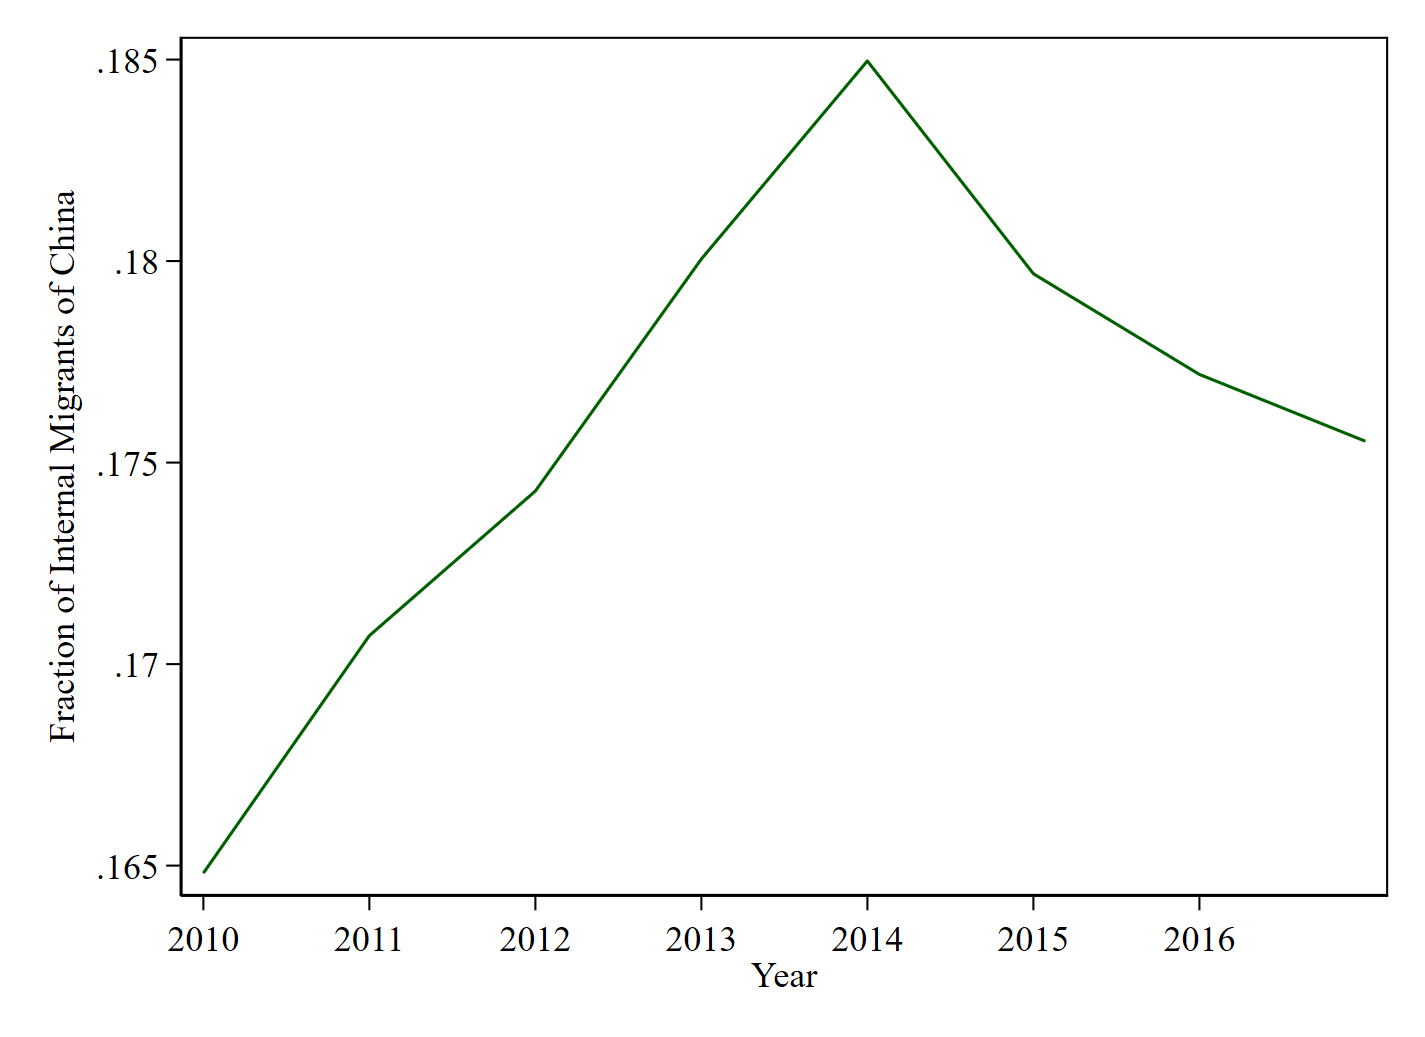
\includegraphics[width=.6\textwidth]{../Analysis/output/fraction_of_internal_migrants.png}
 \caption{Fraction of Internal Migrants, 2010--2016. \vspace{1ex} \\
    {\footnotesize \emph{Notes.} The fraction of internal migrants is calculated as the total number of internal migrants divided by the total population of China. The data is from the National Bureau of Statistics of China (NBSC).}}
  \label{fig:Fraction_of_Internal_Migrants}
\end{figure}
Figure \ref{fig:Fraction_of_Internal_Migrants} plots the share of internal migrants in China's total population in between 2010 and 2016 using National Bureau of Statistics data. The share increased from 16.5\% in 2010 to a peak of 18.5\% in 2014, then slightly declined to approximately 17.6\% by 2016. The post-2014 dip lines up with two landmark hukou-reform announcements—November 2013's communique on “comprehensive and deep reforms” and the State Council's July 2014 Guiding Opinions on Further Deepening the Household-Registration System Reform—which altered migrants' registration incentives. The analysis period (2010--2016) corresponds to consistent availability in both the migration and patent databases.

\subsection{Data Processing}\label{sec:dataprocess}
The processing begins with the immigrant data. First, I harmonise the disparate questionnaires of CMDS, since some definitions of variables are different in different waves.
I merge the CMDS migration data with the CNIPA patent citation records at the prefecture-city level using standardised city codes from the National Bureau of Statistics. Of the initial 292 prefecture-level cities in the migration data, 260 match to patent records. The remaining 32 cities are excluded due to missing or inconsistent identifiers, most of which are small, newly created, or statistical-only administrative units.

Notably, the year associated with each record was shifted backward by one compared to the actual survey wave year. This adjustment accounts for the fact that the CMDS surveys are conducted in the first quarter of each wave year but use samples drawn from the China Migrant Population Information System in the preceding year. This ensures that immigrants' data are consistent with cities' data from 2010 through 2016.
The data is aggregated by weights to the city--year level, resulting in each observation representing a particular city in a specific year. The data include the number of migrants from province $o$. Migration origins are measured at the province level because the CMDS identifies migrants' province of origin but not their prefecture or county. Data also includes characteristics of these migrant flows, such as average years of education, male share, and rural hukou share. I also compute the number of high-skilled migrants, defined as those with education above the college level, and the number of recent migrants, defined as those who migrated within the past year.

The second step involves processing the patent data. The patent dataset comprises all patents granted in China from 2010 to 2016, merged with citation information of other patents referenced by each patent. Key variables include the patent number, date of grant, and city of grant for each patent, alongside corresponding details of the cited patents.
Citations originating from the same city or the same province as the cited patent are excluded to focus on interprovincial knowledge flows. Intra-provincial citations are more likely to reflect localised spillovers or firm-level self-citations, which are conceptually distinct from the migration-driven interregional diffusion I study. Moreover, because my shift-share instrument is defined using cross-province migrant origins, including within-province citations would add noise without contributing to identification.
Subsequently, the data are aggregated to the city--year level, resulting in each observation representing a particular city in a specific year. Patents are categorized into three types: design, invention, and utility. However, design patents, which protect the visual appearance of products, are excluded from the analysis due to their minimal relevance to knowledge inflow and notably lower citation rates. The analysis thus centers on innovation and utility patents, which are inherently tied to technological advancements and knowledge transfer.
I also categorize the citations into self-citations and others.

Finally, I combine data of immigrants, patent and city-level controls to get the city panel.
Since this research focuses on internal migration within mainland China, all data sources exclude Hong Kong, Macao, and Taiwan regions.  Cities without consistent yearbook records or with missing migration or patent data (predominantly smaller prefectures in western China) are excluded to maintain comparability and reduce measurement error. The final panel contains 260 prefecture-level cities across 31 provinces and approximately 12,000 to 14,000 observations. The sample accounts for over 85\% of China's total population in 2015 (around 1.2 billion out of 1.4 billion), ensuring that the analysis captures the vast majority of national economic activity. 

\subsection{Data Description} \label{sec:description}

\begin{table}[!htbp]
 \centering 
 \resizebox{\textwidth}{!}{
   {
\def\sym#1{\ifmmode^{#1}\else\(^{#1}\)\fi}
\begin{tabular}{l*{1}{cccccc}}
\toprule
                    &\multicolumn{6}{c}{}                                                         \\
                    &        Mean&      Median&    St. Dev.&         Min&         Max&        Obs.\\
\midrule
Fr. immigrants      &       0.016&       0.002&       0.058&       0.000&       1.257&       14691\\
Fr. high-skill immigrants&       0.002&       0.000&       0.009&       0.000&       0.298&       14691\\
Fr. recent immigrants&       0.005&       0.001&       0.022&       0.000&       0.502&       14691\\
Fr. recent high-skill imm.&       0.000&       0.000&       0.003&       0.000&       0.096&       14691\\
City population (10,000)&     530.510&     430.590&     432.743&      19.500&    3392.000&       14691\\
Predicted population& 5403895.415& 4383702.500& 4453052.371&  192554.844&35175540.000&       12197\\
Population density  &     507.668&     436.000&     393.867&       5.000&    2648.000&       12819\\
Citation            &       4.619&       4.533&       1.982&       0.693&      11.632&       14193\\
Invention           &       4.585&       4.500&       1.984&       0.000&      11.624&       14193\\
Utility             &       1.499&       1.099&       1.521&       0.000&       6.944&       14193\\
GDP per capita      &   58018.995&   52143.000&   34284.605&    5304.000&  256877.000&       14626\\
Industrial added value/GDP&       0.481&       0.493&       0.105&       0.149&       0.897&       14660\\
Student ratio       &       0.031&       0.022&       0.030&       0.000&       0.129&       12751\\
Average education years&       9.247&       9.428&       2.570&       0.000&      18.000&       14691\\
Rural hukou ratio   &       0.769&       0.862&       0.269&       0.000&       1.000&       14691\\
Male share          &       0.562&       0.550&       0.235&       0.000&       1.000&       14691\\
Average age         &      33.875&      33.952&       5.395&      14.000&      83.000&       14691\\
\bottomrule
\end{tabular}
}

   }
 \caption{Summary Statistics \vspace{1ex} \\ 
   {\footnotesize \emph{Notes.} The variable \emph{Fr.immigrants} is calculated as the number of immigrants from province $o$ divided by the population of city $d$. \emph{Fr.high-skill immigrants} and \emph{Fr.recent immigrants} represent the fractions of high-skilled migrants and recent arrivals, respectively. \emph{Citation}, \emph{Invention}, and \emph{Utility} are the logarithms of 1 plus the number of backward citations for all patents, invention patents, and utility patents, respectively. City-level covariates include total population, population density, GDP per capita, industrial added value as a share of GDP, and the student ratio. Migrant characteristics include average years of education, rural hukou ratio, male ratio, and average age. }}
 \label{tab:summary}
\end{table}

Table \ref{tab:summary} shows that migrant inflows are small on average but highly skewed across cities: immigrants account for about 1.6\% of city populations, with high-skilled and recent arrivals forming much smaller fractions. 
Immigrants share can exceed 1 because the denominator uses the registered (hukou) population of city d at time t, while the numerator counts migrant residents without local hukou living/working in d In cities with large floating populations, the migrant stock can be larger than the registered population.
City characteristics vary widely, with population ranging from under one million to over thirty million and GDP per capita spanning 5,000 to 250,000 RMB, reflecting stark regional inequality. Migrants are predominantly rural (mean rural hukou share of 77\%), relatively young (average age 34), and male-skewed (average male share 56\%). Knowledge inflows, measured through backward citations, also display strong heterogeneity: invention patents dominate, while utility models remain limited, consistent with their incremental nature. Overall, the statistics highlight both the uneven distribution of migrants and the concentration of knowledge flows in a few hubs, underscoring the need for a causal design that accounts for heterogeneity across cities and migrant types.

% 2010
\begin{figure}[!htbp]
 \centering
 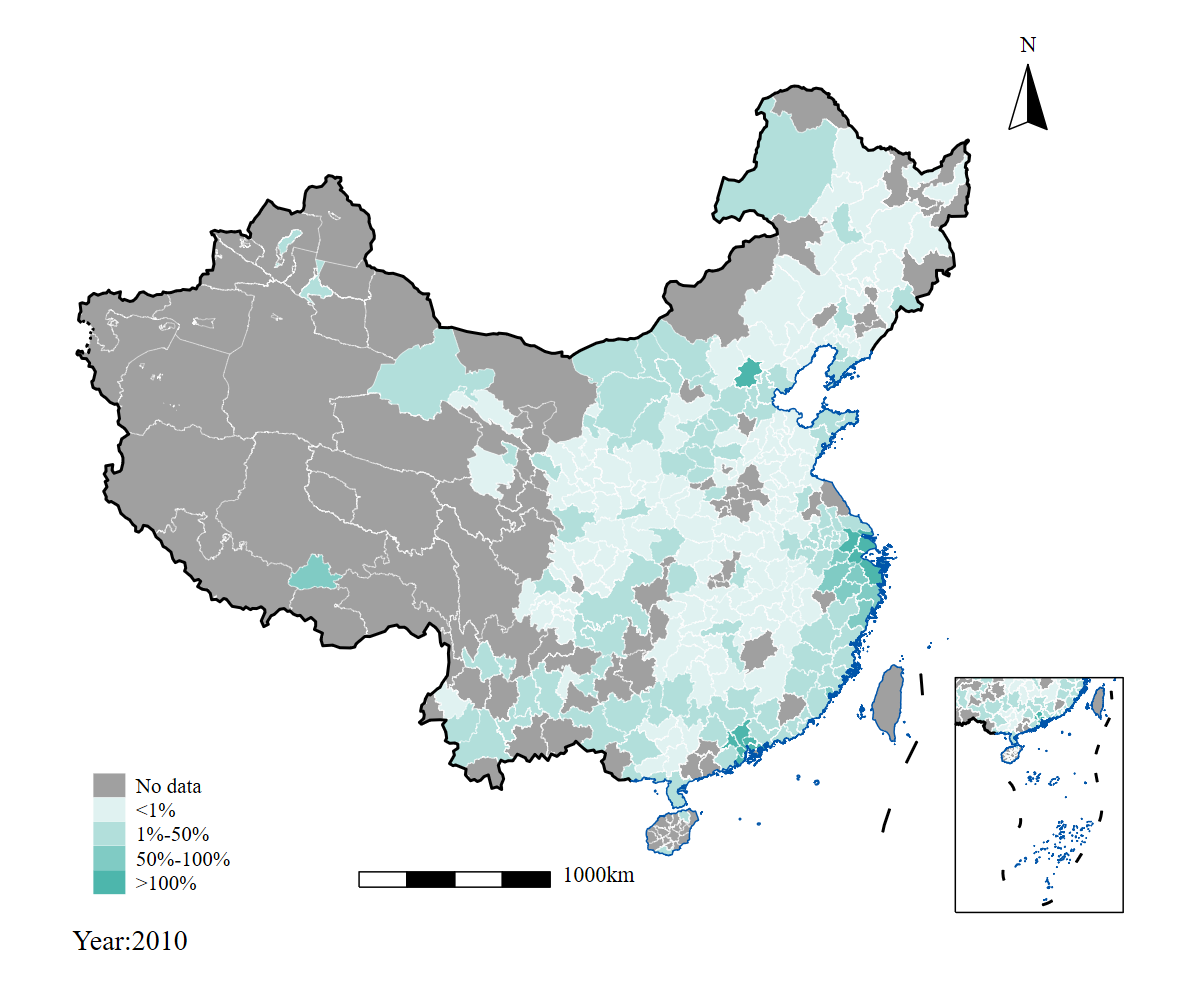
\includegraphics[width=0.65\textwidth]{../Analysis/output/figure_immgrants_share_2010.png}
 \caption{Fraction of \emph{Aggregated} Immigrants in Cities, 2010 \vspace{1ex} \\ 
   {\footnotesize \emph{Notes.} The metric plotted is each city's fraction of the \emph{sum of immigrants whose province of origin differs from the destination city} relative to that city's total predicted resident population in the given year, which is an aggregate of \emph{Fr. immigrants} in Table \ref{tab:summary}. Grey areas indicate cities with no available data.}}
 \label{fig:2010}
\end{figure}

\begin{figure}[!htbp]
 \centering
 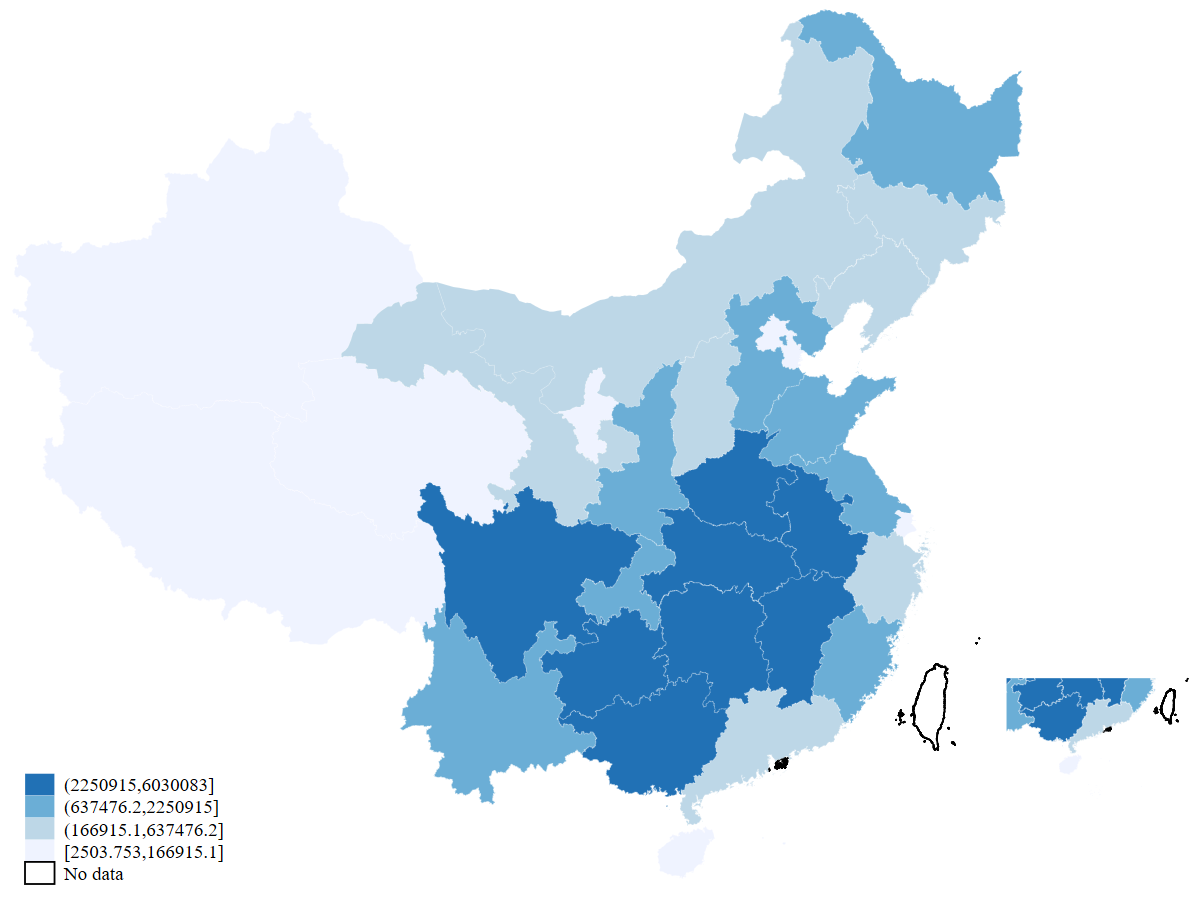
\includegraphics[width=0.65\textwidth]{../Analysis/output/migration_origin.png}
 \caption{Mean Number of Migrants from Origin Provinces \vspace{1ex} \\ 
   {\footnotesize \emph{Notes.} The metric plotted is the average of number of emigrants departing from each province during 2010--2016. White areas indicate provinces with no available data.}}
 \label{fig:origin}
\end{figure}

Figure \ref{fig:2010} illustrates the spatial distribution and temporal evolution of immigrant fractions across cities in 2010. Initially, in 2010, a higher concentration of immigrants exceeding 50\% of the local population was primarily evident in the eastern coastal regions, particularly in the Yangtze River Delta, Pearl River Delta areas and Beijing, indicating these regions' attractiveness due to economic opportunities and urbanization.
The fraction of immigrants continues to follow the same spatial pattern, reflecting diffusion from coastal metropolitan cities to interior urban centres.
Western provinces and remote regions consistently exhibited low immigrant fractions (less than 1\%) or had no available data (shown as grey areas in the map), underscoring persistent regional disparities in economic development and urban appeal.
Figure \ref{fig:origin} visualizes the average number of emigrants departing from each province during the period from 2010 to 2016. The map shows a clear spatial pattern that provinces in central and eastern China exhibit the highest average outflows of migrants, as indicated by the darkest blue shading. In contrast, provinces in western China, such as Tibet and Qinghai, show low average emigration. Coastal regions like Guangdong and Fujian also show moderately high levels of emigration, which may reflect both inter-provincial movement and intra-regional labour mobility. The pattern indicates that internal migration in China is heavily shaped by regional economic conditions and population base, with central provinces playing a key role as origin regions in China's migration landscape. 
Overall, these maps illustrate the dynamic patterns of internal migration in China, marked by sustained inflows to coastal regions and outflows from inland areas. These trends are driven by shifting economic opportunities, infrastructure development, and urbanization policies.


\section{Empirical Strategy} \label{sec:empirical} 

In this section, I introduce the baseline estimating equation (section \ref{sec:baseline}), construct the instrument for immigration (section \ref{sec:instrument}), and the two-stage least squares equations (section \ref{sec:2sls}).

\subsection{Baseline Estimating Equation}\label{sec:baseline}

My goal is to estimate the effect of internal migration on knowledge inflow in China. To do so, I estimate the following equation: 

\begin{equation}
 Y_{dt}=\beta imm_{dt}+\alpha_d+\alpha_t+X_{dt}+u_{dt}
\end{equation}

where $Y_{dt}$ is the knowledge inflow into city $d$ from other provinces in year $t$, measured as the log of 1 plus number of backward citations made by patents granted to inventors in city $d$ that reference patents whose first inventor is located outside city $d$. When I examine province-city links, I sum only citations to patents whose first inventor is in province $p\neq \text{}(d)$. Backward citations capture the sources a new patent builds on, hence the inflow of knowledge. $imm_{dt}$ is the fraction of immigrants in city $d$ in year $t$ (or migrant stock/population), it could be seen as the strength of the knowledge transfer network. $\alpha_d$ and $\alpha_t$ are city fixed effects and year fixed effects, respectively. $X_{dt}$ is a vector of control variables. The coefficient $\beta$ captures the correlation between the fraction of immigrants and knowledge inflow.

However, the simple OLS is unlikely to recover the causal effect and even with fixed effects that absorb city-specific trends. A key challenge in studying migration's effects is that flows of migrants are not random; people's decision to move and their destinations depend on economic opportunities and local conditions. To address this, recent studies frequently adopt quasi-experimental methods, including difference-in-difference \citep{fogedImmigrantsEffectNative2016,bernsteinContributionHighSkilledImmigrants2022a} and instrumental variable \citep{cardImmigrantInflowsNative2001,lewisImmigrationSkillMix2011,tabelliniGiftsImmigrantsWoes2019,dustmannFreeMovementOpen2019,giulianoSeedsIdeologyHistorical2020}. The influential instruments in recent studies often follow a shift-share logic: they interact historical migrant networks with exogenous origin-specific shocks, generating plausibly random variation in local inflows. 

In my study, there are two main issues. First is omitted variable bias, when the omitted variable is correlated with the fraction of immigrants and is a determinant of the knowledge inflow. Unobserved shocks may both attract migrants and raise citations. High-speed railway improves intercity access, which increases intercity migration flows and talent reallocation; at the same time, it also boosts intercity innovation collaboration \citep{wangHighspeedRailUrban2024}. Classic and recent work shows knowledge spillovers are geographically localized: places dense in R\&D labs and universities generate (and receive) more patent citations \citep{jaffeGeographicLocalizationKnowledge1993,kwonKnowledgeSpilloversPatent2022}. If data are available, this issue can be solved by adding the variable into controls. A further problem is that many of variables are unobservable. Second is reverse causality. Migration implies knowledge inflow and knowledge inflow implies migration. For example, \cite{moserGermanJewishEmigres2014} document that during the Nazi persecution of Jewish scientists, emigration destinations were strongly influenced by pre-existing professional networks, illustrating how established knowledge hubs can act as powerful pull factors for migrant flows.


\subsection{Shift-share Instrument Construction}\label{sec:instrument}

To recover the causal effect, identification strategy is needed. Thanks to the seminal work of \citep{cardImmigrantInflowsNative2001,borusyakQuasiExperimentalShiftShareResearch2022}, I construct a shift-share instrument. The motivation for using a shift-share instrument is that the treatment measures the changes of the fraction of immigrants in a city over time and the treatment can be decomposed into some start-of-period share and over-time shifts. The instrument $Z_{dt}$ is constructed as follows:
\begin{equation}
 Z_{dt}=\frac{1}{\hat{Pop}_{dt}}\sum_{o \neq \text{prov}(d)} s_{od}^{2010} g_{ot}^{-d}
\end{equation}
where $\hat{Pop}_{dt}$ is the predicted registered population of city $d$ in year $t$,$s_{od}^{2010}$ is the share of province $o$'s emigrants that live in city $i$ in 2010, and $g_{ot}^{-d}$ is the year-$t$ total number of migrants leaving province $o$, excluding those who settle in city $d$. This exclusion follows \cite{tabelliniGiftsImmigrantsWoes2019} that shift-share instrument was constructed in a "leave-out" version, by excluding immigrants from each province who eventually settled in a given city. Lastly, both $g_{ot}$ and $s_{od}$ exclude migrants internal same province to coincide with the patent citation data. 

The validity of the shift-share instrument rests on three conditions: relevance, exogeneity (exclusion restriction), and monotonicity.

First, relevance requires that the instrument is sufficiently correlated with the endogenous regressor so that the first-stage relationship is strong. In this case, the shift share instrument is sufficiently correlated with the migrant share in city $d$. I report the first-stage coefficients and Kleibergen-Paap $F$-statistics in Section \ref{sec:first}.

Second, exogeneity requires that the instrument is uncorrelated with the structural error term in the second-stage equation. In the shift-share framework, this means that at least one of its components—either the base-period shares or the subsequent shocks—is plausibly exogenous. I adopt a shift-driven design: the shares $s^{2010}_{od}$, measuring the fraction of migrants from origin province $o$ living in city $d$ in 2010, are fixed in the base year, while the annual shocks $g^{-d}_{ot}$—the number of migrants leaving origin $o$ in year $t$, excluding those settling in city $d$—are assumed to be exogenous to contemporaneous, city-specific shocks to knowledge inflow. This “leave-out” formulation further removes mechanical correlation between the instrument and the error term. In the Chinese context, shocks to outmigration from each province—driven by factors such as hukou reform announcements, large-scale infrastructure roll-outs, or province-specific economic fluctuations—are plausibly unrelated to unobserved, city-level determinants of patent citations in unrelated destinations. The base-year shares simply capture each city's historical exposure to these origin-specific shocks. Additionally, I use the predicted population as the denominator in constructing instrument and calculating fraction of immigrants because city population may itself be an outcome of immigration. The predicted city population is calculated as $\hat{Pop}_{dt}=Pop_{d,2010} \times growth_t^{-p}$, where $Pop_{d,2010}$ is 2010 city population and $growth_t^{-p}=\frac{Pop_t^{-p}-Pop_{t-1}^{-p}}{Pop_{t-1}^{-p}}$ is the population growth rate between year $t$ and $t-1$, constructed leaving out the province of city $d$.

Finally, monotonicity requires that, for each city-origin pair, the migration shock affects the migrant share in the same direction for all units (no “defiers”). Given that $g^{-d}_{ot}$ is an aggregate outflow measure, this condition is plausible in our setting.

However, assumptions can still be violated for two main reasons. To deal with these concerns and ensure the validity of the instrument, some robustness checks will be applied.
First, if the characteristics of cities that attracted early immigrants (from each sending province) had persistent, confounding effects on migration patterns as well as on changes in the outcomes of interest. To solve this concern, I first include city fixed effects to partially out city specific trends. I also control for 2010 migrant shares directly to avoid comparing cities with different baseline levels of immigration from a given province.
The second reason why the identifying assumption can be violated is that outmigration from each province might not be independent of cross-city pull factors systematically related to 2010 settlers' province of origin. To address this concern, I use alternative instruments and check pre-trends in later section \ref{sec:robustness}.

\subsection{First Stage Regression}\label{sec:first}

The first-stage estimates in Table \ref{tab:first_stage} provide strong evidence that the shift-share variable $Z$ is a powerful and stable predictor of a city's immigrant share. Across all specifications, the coefficient on $Z$ remains tightly clustered around 28,000 and highly significant at the 1\% level. The stability of this relationship after progressively adding controls and fixed effects suggests that the instrument's explanatory power is not driven by omitted fundamentals such as city size, density, or economic structure.

This gradual decline is expected, as the added covariates absorb some of the variation initially captured by the instrument. The fact that the coefficient remains robust reinforces that $Z$ continues to reflect exogenous supply shocks rather than demand-driven immigrant flows. Instrument strength is confirmed by the Kleibergen-Paap rk Wald $F$-statistics, which range from 251 to 2082, far exceeding the conventional weak-instrument threshold of 10.
Such values imply that finite-sample bias in the second stage is negligible and that statistical inference based on standard $t$-statistics is reliable.


\begin{table}[htbp!]
  \centering 
  \resizebox{\textwidth}{!}{
    \begin{tabular}{lccccc} \hline
 & (1) & (2) & (3) & (4) & (5) \\
VARIABLES & Fr. immigrants & Fr. immigrants & Fr. immigrants & Fr. immigrants & Fr. immigrants \\ \hline
 &  &  &  &  &  \\
Zpredict & 29,462*** & 29,097*** & 28,090*** & 27,599*** & 27,514*** \\
 & (645.7) & (779.9) & (799.6) & (790.2) & (800.8) \\
Initial share &  &  & 0.172*** & 0.161*** & 0.162*** \\
 &  &  & (0.0338) & (0.0365) & (0.0368) \\
City population (10,000) &  &  &  & -3.30e-05 & -3.26e-05 \\
 &  &  &  & (2.38e-05) & (2.35e-05) \\
Population density &  &  &  & 4.37e-05** & 4.32e-05** \\
 &  &  &  & (2.00e-05) & (1.95e-05) \\
GDP per capita &  &  &  & 1.99e-08 & 2.19e-08 \\
 &  &  &  & (3.21e-08) & (3.18e-08) \\
Industrial added value/GDP &  &  &  & 0.00513 & 0.00512 \\
 &  &  &  & (0.00771) & (0.00774) \\
Student ratio &  &  &  & 0.0121 & 0.0116 \\
 &  &  &  & (0.0119) & (0.0118) \\
Average education years &  &  &  &  & -0.000134 \\
 &  &  &  &  & (0.000165) \\
Rural hukou ratio &  &  &  &  & 0.00398*** \\
 &  &  &  &  & (0.00125) \\
Male share &  &  &  &  & 0.000348 \\
 &  &  &  &  & (0.000322) \\
Average age &  &  &  &  & 9.22e-05*** \\
 &  &  &  &  & (3.47e-05) \\
 &  &  &  &  &  \\
City FE & No & Yes & Yes & Yes & Yes \\
Time FE & No & Yes & Yes & Yes & Yes \\
~ & ~ & ~ & ~ & ~ & ~ \\
Number of Observations & 12197 & 12195 & 12195 & 10279 & 10279 \\
Number of Cities & 268 & 266 & 266 & 265 & 265 \\
 $ F-stat$ & 2082.043 & 1392.117 & 706.123 & 274.556 & 251.761 \\ \hline
\end{tabular}

  }
  \caption{Instrument Relevance: First-Stage Regression of Immigrant Share on Shift-Share Instrument \vspace{1ex} \\ 
  {\footnotesize \emph{Notes.} The dependent variable in all columns is Fr. immigrants, the share of migrants from other provinces in city d at time t. The key regressor Z is the shift-share instrument that interacts the baseline (2010) province-of-origin migrant shares with year-specific province inflow shocks. Columns (1)-(6) successively add covariates: the initial immigrant share, total city population, population density, GDP per capita, the ratio of industrial value added to GDP, the college-student ratio, average education years, rural hukou, gender and average age. Robust standard errors clustered by city. City and year fixed effects are included from column (2) onward. Robust standard errors clustered at the city level. The reported \emph{F-stat} test the joint relevance of the instrument(s). 
 \\ $^{***}$: $p < 0.01$, $^{**}$: $p < 0.05$, $^{*}$: $p < 0.1$.}}
 \label{tab:first_stage}
\end{table}

Figure \ref{fig:first_stage} plots the actual fraction of immigrants against the value predicted by the shift-share instrument. The cloud hugs a line with a tight, linear fit, indicating that the instrument tracks realized inflows closely. The slope is near one and dispersion is modest except for a handful of high-inflow cities in the upper-right corner and a few small negatives on the left, which likely reflect sampling noise in very low-migration places. 
Combined with the high first-stage F-stats reported in Table \ref{tab:first_stage}, the figure visually confirms instrument relevance and the absence of major leverage points.

Overall, the first-stage regressions validate the relevance assumption and provide a strong foundation for causal interpretation of the second-stage results.

\begin{figure}[htbp!]
  \centering
  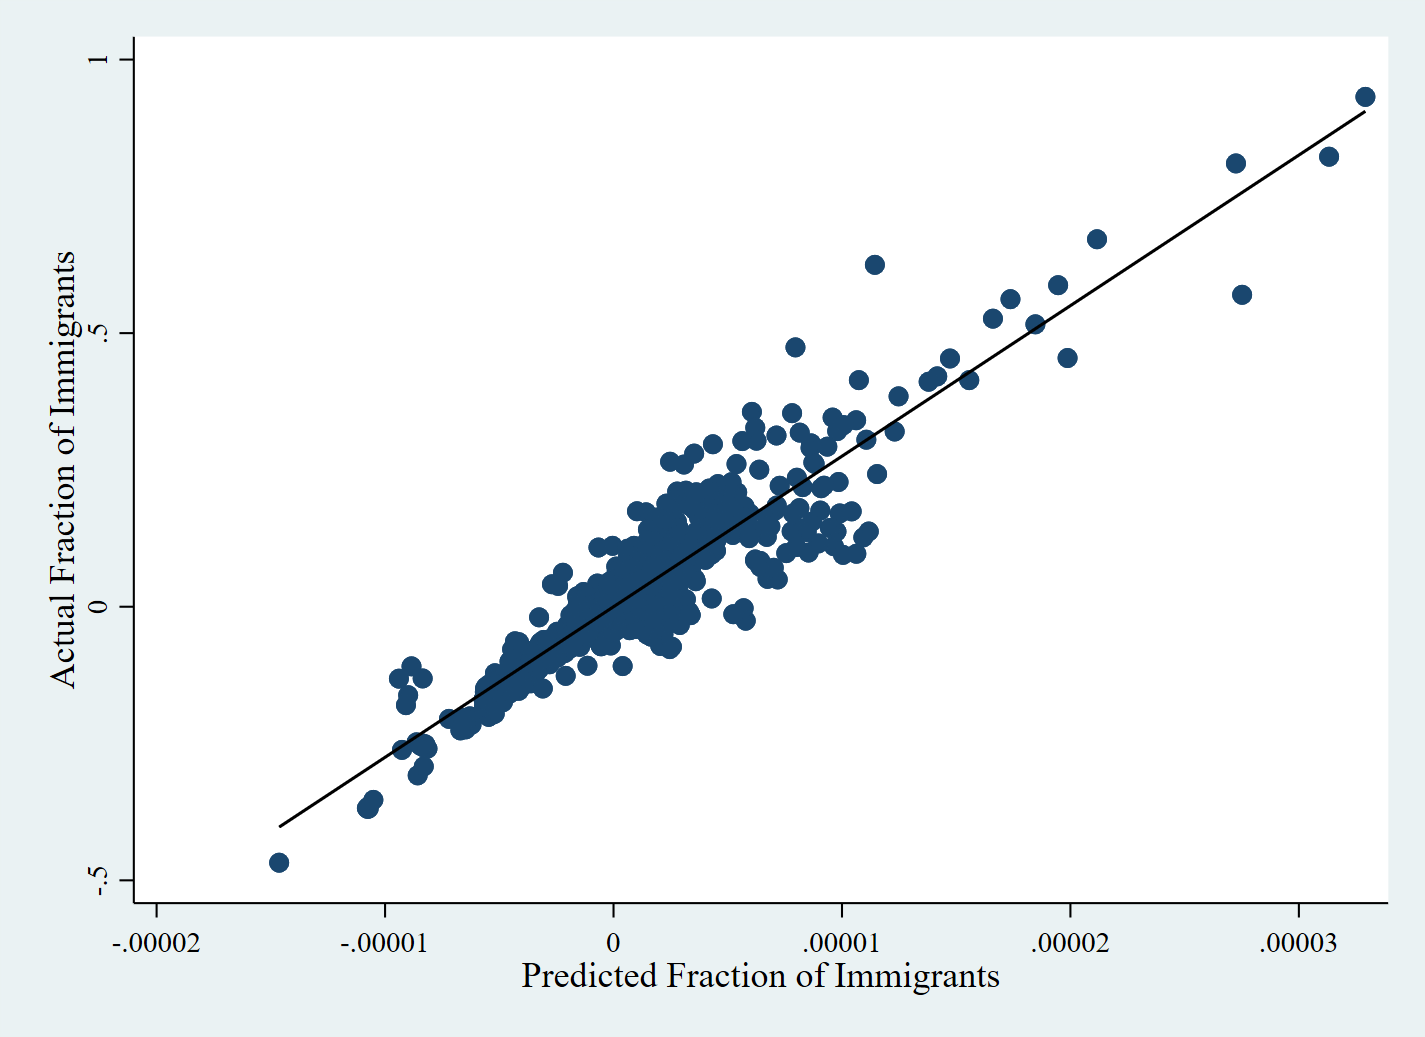
\includegraphics[width=.6\textwidth]{../Analysis/output/First_stage_actual_vs_predicted_immigration.png}
  \caption{First stage actual vs predicted immigration}
  \label{fig:first_stage}
\end{figure}


\subsection{Two-Stage Equations}\label{sec:2sls}

Then I can apply the instrument to estimate the effect using the following two-stage least squares (2SLS) regression:
\begin{equation}
 imm_{dt}=\pi Z_{dt}+\alpha_d+\alpha_t+X_{dt}+e_{dt}
\end{equation}
\begin{equation}
 Y_{dt}=\beta\widehat{imm_{dt}}+\alpha_d+\alpha_t+X_{dt}+\epsilon_{dt}
\end{equation}

where $imm_{dt}$ is the fraction of immigrants of city $d$ in year $t$, $Z_{dt}$ is the shift-share instrument, $\widehat{imm_{dt}}$ is the predicted value of fraction of immigrants. $\pi$ is the first stage coefficient. $\beta$ is the effect of immigrants on knowledge inflow. 

Control variables are correlated with both the fraction of immigrants and the number of citations received by patents and are employed to mitigate confounding effects and omitted variable bias. I include a comprehensive set of control variables, categorized into city-level characteristics, migrant flow characteristics, and the initial share of immigrants. City-level controls encompass population, population density, GDP per capita, industrial added value, and the proportion of college-educated residents. Controlling for population and population density ensures comparability across cities of varying sizes, which may otherwise distort the impact of immigration. GDP per capita accounts for differential city attractiveness influencing both immigrant settlement decisions and patent citations. Industrial added value captures variations in economic structure, while the proportion of college-educated residents reflects differences in human capital and innovation potential across cities. Migrant flow characteristics include average years of education, age composition, gender distribution, and hukou status, which collectively measure the capacity of migrants to facilitate knowledge inflow.


\section{Results} \label{sec:result}

This section presents the empirical analysis results, including both OLS and 2SLS estimates of the primary research question—the effect of immigrants on knowledge inflows within China. Particular attention is given to discussing the differences between the OLS and 2SLS estimates (Section \ref{sec:main_result}). 
Subsequently, I examine the effects specifically attributable to high-skilled immigrants and recent immigrants (Section \ref{sec:high_skill}). 
Furthermore, the heterogeneity of the immigrant effect across different regions is discussed (Section \ref{sec:region}).
Finally, I explore the mechanisms of knowledge flow by distinguishing between invention and utility patents and through self-citations (Section \ref{sec:innovation_and_utility}). 


\subsection{The Effect of Immigration on Knowledge Inflow}\label{sec:main_result}
\begin{table}[!htbp]
  \centering  
  \resizebox{\textwidth}{!}{
      \begin{tabular}{lccccc} \hline
 & (1) & (2) & (3) & (4) & (5) \\
VARIABLES & Citation & Citation & Citation & Citation & Citation \\ \hline
 &  &  &  &  &  \\
Fr. immigrants & 6.184*** & 1.138*** & 1.066*** & 0.950*** & 1.148*** \\
 & (1.252) & (0.383) & (0.290) & (0.271) & (0.276) \\
 &  &  &  &  &  \\
Initial Share & No & No & Yes & Yes & Yes \\
City Controls & No & No & No & Yes & Yes \\
Immigrants Characteristics & No & No & No & No & Yes \\
City FE & No & Yes & Yes & Yes & Yes \\
Time FE & No & Yes & Yes & Yes & Yes \\
~ & ~ & ~ & ~ & ~ & ~ \\
Number of Observations & 11963 & 11961 & 11961 & 10060 & 10060 \\
Number of Cities & 270 & 268 & 268 & 264 & 264 \\
 $ R^2$ & 0.034 & 0.766 & 0.766 & 0.759 & 0.772 \\ \hline
\end{tabular}

  }
  \caption{OLS: The effect of immigrants on knowledge inflow\vspace{1ex} \\ 
  {\footnotesize \emph{Notes.} This table reports OLS results of the effect of immigrants on knowledge inflow. Fr. immigrants is the fraction of immigrants of city population  (immigrants stock/registered population), Citation is the natural logarithm of 1 plus backward citation. Column 1 report the raw OLS result. Column 2 adds city and time fixed effect. Column 3 adds controlling share which is the initial total immigrant share. Column 4 adds city-level controls. Column 5 adds controls for the characteristics of immigrants. Standard errors clustered at the city level.
 \\ $^{***}$: $p < 0.01$, $^{**}$: $p < 0.05$, $^{*}$: $p < 0.1$.}}
 \label{tab:main_ols}
\end{table}


\begin{table}[!htbp]
  \centering 
  \resizebox{\textwidth}{!}{
    \begin{tabular}{lccccc} \hline
 & (1) & (2) & (3) & (4) & (5) \\
VARIABLES & Citation & Citation & Citation & Citation & Citation \\ \hline
 &  &  &  &  &  \\
Fr. immigrants & 5.218*** & 0.657** & 0.484* & 0.405* & 0.648*** \\
 & (0.974) & (0.308) & (0.250) & (0.221) & (0.220) \\
 &  &  &  &  &  \\
Initial Share & No & No & Yes & Yes & Yes \\
City Controls & No & No & No & Yes & Yes \\
Immigrants Characteristics & No & No & No & No & Yes \\
City FE & No & Yes & Yes & Yes & Yes \\
Time FE & No & Yes & Yes & Yes & Yes \\
~ & ~ & ~ & ~ & ~ & ~ \\
Kleibergen–Paap F-stat & 2080.58 & 1408.85 & 1250.83 & 1232.73 & 1193.48 \\
Number of Observations & 11932 & 11930 & 11930 & 10053 & 10053 \\
Number of Cities & 267 & 265 & 265 & 263 & 263 \\
 $ R^2$ & 0.033 & 0.003 & 0.003 & 0.006 & 0.062 \\ \hline
\end{tabular}

  }
  \caption{2SLS: The effect of immigrants on knowledge inflow\vspace{1ex} \\ 
  {\footnotesize \emph{Notes.} This table reports 2SLS results of the effect of immigrants on knowledge inflow. Fr. immigrants is the fraction of immigrants of city population (immigrants stock/registered population), Citation is the natural logarithm of 1 plus backward citation. Column 1 report the raw 2SLS result. Column 2 adds city and time fixed effect. Column 3 adds controlling share which is the initial total immigrant share. Column 4 adds city level controls. Column 5 adds controls for the characteristics of immigrants. Kleibergen-Paap rk F-stat reported for IV models. Standard errors clustered at the city level. 
 \\ $^{***}$: $p < 0.01$, $^{**}$: $p < 0.05$, $^{*}$: $p < 0.1$.}}
 \label{tab:main_2sls}
\end{table}

The results reported in Tables \ref{tab:main_ols} and \ref{tab:main_2sls} provide complementary perspectives on the relationship between immigrant inflows and patent-based knowledge inflow across Chinese cities, measured as the fraction of immigrants of cities population and logarithm of 1 plus number of backward citations in patents granted to inventors in city that reference patents whose registration location in another province.

The initial OLS regressions presented in Table \ref{tab:main_ols} indicate a significant positive correlation between immigrant inflow shares and the logarithm of 1 plus backward patent citations. The coefficient of raw OLS collapses from 6.184 to 1.138 once I use the fixed effect model including city and year fixed effects, implying that time-invariant city characteristics and nationwide shocks drove most of the upward bias. 
After adding initial immigrant stock, density, GDP, industrial structure, student ratio reduces the estimate modestly but leaves it significant, and further controls for migrant-flow composition average education years, age, rural-hukou share and gender, estimate stabilizes around 1.148 and remains highly significant, suggesting that a one-percentage-point increase in the immigrant share correlates with a 1.148 percent increase in citations. The coefficient changes only modestly when adding observed city and migrant characteristics, indicating that these particular covariates account for little of the raw OLS-FE difference. 

However, the larger gap between OLS and 2SLS estimates points to non-negligible endogeneity, consistent with migrants sorting into cities experiencing unobserved innovation shocks. The most straightforward interpretation is positive selection: cities already on a trajectory of faster knowledge inflow attracted more immigrants due to their favourable prospects. As a result, the OLS estimates capture not only the causal effect of immigration but also the influence of unobserved innovation-friendly attributes—such as export \citep{pengEffectsExportGrowth2025}, digital technological advances \citep{luDigitalEconomyUrban2025}, industrial robots \citep{bianEffectsRobotsInternal2024} and land redevelopment \citep{wangLandRedevelopmentMigrant2023}.
Once I replace endogenous inflows with variation driven by origin-province supply shocks, the coefficient falls to a more credible causal magnitude. Supporting this interpretation, the OLS estimate drops from 6.184 to 1.138 after controlling for city and year fixed effects, suggesting that time-invariant favourable city characteristics and nationwide shocks had inflated the naive OLS estimate.
The second reason is OLS and 2SLS estimate average treatment effect and local average treatment effect (LATE), that emphasis different aspects. The 2SLS recovers the LATE for complier cities—those whose immigrant share moved because of province-level supply shocks. These compliers may differ systematically from always-takers or never-takers. For instance, if marginal immigrants induced by origin shocks tend to settle in less developed cities, the IV effect of knowledge inflow could be larger than the average effect captured by OLS. This is because OLS places more weight on cities that are sources of innovation, which typically have high knowledge outflows but relatively low inflows. I gauge the heterogeneity by re-estimate OLS and 2SLS separately for coastal, central, and western prefectures in Section \ref{sec:region}.
The third reason is the potential biased estimate of 2SLS which would be caused by violation of the assumption of exclusion. It is possible that the immigrant share was actually influenced by emigrants shocks to cities with higher knowledge inflow. I test the exclusion assumption in Section \ref{sec:robustness} by checking the pre-trends, covariates balance checks and using alternative instruments.

Therefore Table \ref{tab:main_2sls} instruments the immigrant share with the shift-share variable described in Section \ref{sec:instrument}.
In these IV regressions, the estimates remain significantly positive, though the magnitudes shrink to approximately half the size observed under OLS specifications. Specifically, the most comprehensive 2SLS specification yields a coefficient of 0.648, indicating that a one-percentage-point increase in immigrant share leads to about a 0.648 percent increase in backward citations. This attenuation relative to OLS suggests that approximately half of the naive OLS correlation reflects endogenous sorting of migrants into innovation-rich cities, yet confirms that a substantial, causally interpretable relationship persists.

The stability of results across progressively richer specifications in both OLS and IV settings supports the credibility of this relationship. Additionally, the consistent significance of the IV estimates, despite their diminished magnitude, provides robust evidence that immigration actively promotes the spatial diffusion of knowledge rather than merely following it. 

\subsection{Heterogeneity by Migrant Type}\label{sec:high_skill}
\begin{table}[!htbp]
  \centering 
  \resizebox{\textwidth}{!}{
  \begin{tabular}{lcccccc} \hline
 & (1) & (2) & (3) & (4) & (5) & (6) \\
VARIABLES & Citation & Citation & Citation & Citation & Citation & Citation \\ \hline
 &  &  &  &  &  &  \\
Fr. high skilled immigrants & 39.13*** & 5.020** & 3.844* & 3.274* & 3.268* & 3.245* \\
 & (13.95) & (2.400) & (1.955) & (1.796) & (1.799) & (1.792) \\
Initial share &  &  & 0.762 & 0.929 & 0.932 & 0.934 \\
 &  &  & (1.322) & (1.308) & (1.307) & (1.307) \\
City population (10,000) &  &  &  & 0.00223** & 0.00234** & 0.00219* \\
 &  &  &  & (0.00109) & (0.00112) & (0.00113) \\
Population density &  &  &  & -0.00173*** & -0.00191*** & -0.00187*** \\
 &  &  &  & (0.000572) & (0.000645) & (0.000644) \\
GDP per capita &  &  &  &  & 2.24e-06* & 2.48e-06* \\
 &  &  &  &  & (1.31e-06) & (1.33e-06) \\
Industrial added value/GDP &  &  &  &  & 2.515*** & 2.394*** \\
 &  &  &  &  & (0.766) & (0.771) \\
Student ratio &  &  &  &  &  & 0.146 \\
 &  &  &  &  &  & (0.446) \\
 &  &  &  &  &  &  \\
City FE & No & Yes & Yes & Yes & Yes & Yes \\
Time FE & No & Yes & Yes & Yes & Yes & Yes \\
~ & ~ & ~ & ~ & ~ & ~ & ~ \\
Kleibergen–Paap F-stat & 12.73 & 11.96 & 8.96 & 9.14 & 9.14 & 9.14 \\
Number of Observations & 11932 & 11930 & 11930 & 10101 & 10095 & 10053 \\
Number of Cities & 267 & 265 & 265 & 264 & 263 & 263 \\
 $ R^2$ & 0.037 & 0.004 & 0.004 & 0.005 & 0.007 & 0.007 \\ \hline
\end{tabular}

  }
  \caption{The effect of high skilled immigrants on knowledge inflow\vspace{1ex} \\ 
  {\footnotesize \emph{Notes.} This table reports 2SLS results on the effect of high-skilled immigrants on knowledge inflow. Fr. high skilled immigrants is the fraction of high skilled immigrants of city population, Citation is the natural logarithm of 1 plus backward citation. Column 1 reports the raw 2SLS result. Column 2 adds city and time fixed effect. Column 3 adds controlling share which is the initial total immigrant share. Column 4 adds controlling population density per square kilometer. Column 5 adds 2 economic control GDP per capita and industrial added value normalised by regional GDP. Column 6 adds controlling for college student ratio. Standard errors clustered at the city level.
 \\ $^{***}$: $p < 0.01$, $^{**}$: $p < 0.05$, $^{*}$: $p < 0.1$.}}
 \label{tab:high}
\end{table}
\begin{table}[!htbp]
  \centering 
  \resizebox{\textwidth}{!}{
  \begin{tabular}{lcccccc} \hline
 & (1) & (2) & (3) & (4) & (5) & (6) \\
VARIABLES & Citation & Citation & Citation & Citation & Citation & Citation \\ \hline
 &  &  &  &  &  &  \\
Fr. recent immigrants & 14.33*** & 1.824* & 1.306* & 1.080* & 1.078* & 1.071 \\
 & (3.697) & (0.998) & (0.765) & (0.650) & (0.652) & (0.652) \\
Initial share &  &  & 0.924 & 1.047 & 1.049 & 1.051 \\
 &  &  & (1.319) & (1.300) & (1.299) & (1.299) \\
City population (10,000) &  &  &  & 0.00217** & 0.00227** & 0.00213* \\
 &  &  &  & (0.00105) & (0.00109) & (0.00109) \\
Population density &  &  &  & -0.00163*** & -0.00181*** & -0.00178*** \\
 &  &  &  & (0.000540) & (0.000614) & (0.000613) \\
GDP per capita &  &  &  &  & 2.32e-06* & 2.57e-06* \\
 &  &  &  &  & (1.30e-06) & (1.31e-06) \\
Industrial added value/GDP &  &  &  &  & 2.508*** & 2.388*** \\
 &  &  &  &  & (0.765) & (0.770) \\
Student ratio &  &  &  &  &  & 0.156 \\
 &  &  &  &  &  & (0.445) \\
 &  &  &  &  &  &  \\
City FE & No & Yes & Yes & Yes & Yes & Yes \\
Time FE & No & Yes & Yes & Yes & Yes & Yes \\
~ & ~ & ~ & ~ & ~ & ~ & ~ \\
Kleibergen–Paap F-stat & 71.92 & 83.20 & 75.82 & 84.20 & 84.16 & 84.15 \\
Number of Observations & 11932 & 11930 & 11930 & 10101 & 10095 & 10053 \\
Number of Cities & 267 & 265 & 265 & 264 & 263 & 263 \\
 $ R^2$ & 0.017 & 0.000 & 0.001 & 0.002 & 0.005 & 0.004 \\ \hline
\end{tabular}

  }
  \caption{The effect of recent immigrants on knowledge inflow\vspace{1ex} \\ 
  {\footnotesize \emph{Notes.} This table reports 2SLS results of the effect of recent immigrants on knowledge inflow. Fr. recent immigrants is the fraction of immigrants who move to city within one year, Citation is the natural logarithm of 1 plus backward citation. Column 1 reports the raw 2SLS result. Column 2 adds city and time fixed effect. Column 3 adds controlling share which is the initial total immigrant share. Column 4 adds controlling population density per square kilometer. Column 5 adds 2 economic control GDP per capita and industrial added value normalised by regional GDP. Column 6 adds controlling for college student ratio. Standard errors clustered at the city level.
 \\ $^{***}$: $p < 0.01$, $^{**}$: $p < 0.05$, $^{*}$: $p < 0.1$.}}
 \label{tab:recent}
\end{table}

This subsection investigates whether the aggregate impact previously identified is predominantly driven by high-skill migrants or recent arrivals. High-skill migrants proxy the capacity to transmit codified and tacit knowledge, whereas recent arrivals indicate how quickly migration translates into citation linkages.
I re-estimate the 2SLS model by replacing the overall migrant share with two alternative measures: (i) the fraction of high-skill migrants (those with a college education or above), and (ii) the fraction of migrants who arrived within the last year.  Fixed effects, and the shift-share instrument remain consistent with definitions provided in Section \ref{sec:empirical}. City-level control variables and the initial migrant share are retained. Controls for migrant-flow composition are not included in this analysis, as the focus is explicitly on specific subgroups of immigrants. Standard errors are clustered at the city level.


Table \ref{tab:high} shows a estimated coefficient on the high-skill migrant share.
Interpreted at the mean, a one-percentage-point increase in the high-skill migrant share raises backward citations by 3.245\%. The point estimate is about 5 times larger than the effect of general migrants, indicating that high-skilled migrants possess greater capacity for knowledge transfer. This finding aligns with \cite{baharMigrationKnowledgeDiffusion2018} who find skilled immigrants have about ten times the impact of unskilled immigrants in diffusion production knowledge. 

Table \ref{tab:recent} reveals a positive but comparatively smaller coefficient for recent arrivals. Statistical significance diminishes after introducing full controls.
This suggests that recent migrants are less likely to contribute to knowledge inflow than earlier migrants. This may be due to the fact that recent migrants may not have had enough time to contribute to knowledge inflow, or that they are not as well integrated into the local economy as earlier migrants.


\subsection{Regional Heterogeneity}\label{sec:region}
\begin{table}[!htbp]
  \centering 
  \resizebox{\textwidth}{!}{
  \begin{tabular}{lcccccc} \hline
 & (1) & (2) & (3) & (4) & (5) & (6) \\
VARIABLES & East & Central & West & Exclude east & Exclude west & Exclude central \\ \hline
 &  &  &  &  &  &  \\
Fr. immigrants & 0.480** & 77.86*** & 9.493*** & 10.53*** & 0.552** & 0.581*** \\
 & (0.234) & (25.15) & (1.695) & (2.177) & (0.224) & (0.220) \\
 &  &  &  &  &  &  \\
Initial Share & Yes & Yes & Yes & Yes & Yes & Yes \\
City Controls & Yes & Yes & Yes & Yes & Yes & Yes \\
Immigrants Characteristics & Yes & Yes & Yes & Yes & Yes & Yes \\
City FE & Yes & Yes & Yes & Yes & Yes & Yes \\
Time FE & Yes & Yes & Yes & Yes & Yes & Yes \\
~ & ~ & ~ & ~ & ~ & ~ & ~ \\
Kleibergen–Paap F-stat & 2627.10 & 39.79 & 17.61 & 17.30 & 2703.82 & 1181.97 \\
Number of Observations & 4639 & 2302 & 3112 & 5414 & 6941 & 7751 \\
Number of Cities & 86 & 90 & 87 & 177 & 176 & 173 \\
 $ R^2$ & 0.091 & 0.080 & 0.041 & 0.048 & 0.079 & 0.064 \\ \hline
\end{tabular}

  }
  \caption{Regional Heterogeneity in the Effect of Immigrants on Knowledge Inflow\vspace{1ex} \\ 
  {\footnotesize \emph{Notes.} The dependent variable is the natural log of 1 plus backward patent citations received by city $d$ from other provinces in year $t$. All regressions control for the initial immigrant share, population density, GDP per capita, the ratio of industrial value added to GDP, the college-student ratio, average education years, rural hukou, gender and average age, and include city and year fixed effects. Columns (1)-(3) restrict the sample to eastern, central, and western cities, respectively, while columns (4)-(6) drop each region in turn. Robust standard errors clustered by city.
 \\ $^{***}$: $p < 0.01$, $^{**}$: $p < 0.05$, $^{*}$: $p < 0.1$.}}
 \label{tab:region}
\end{table}

\begin{table}[!htbp]
  \centering 
  \resizebox{\textwidth}{!}{
  \begin{tabular}{lcccccc} \hline
 & (1) & (2) & (3) & (4) & (5) & (6) \\
VARIABLES & East & Central & West & Exclude east & Exclude west & Exclude central \\ \hline
 &  &  &  &  &  &  \\
Fr. immigrants & 1.032*** & 53.87*** & 7.407*** & 8.684*** & 1.104*** & 1.079*** \\
 & (0.250) & (11.94) & (2.039) & (2.413) & (0.258) & (0.266) \\
 &  &  &  &  &  &  \\
Initial Share & Yes & Yes & Yes & Yes & Yes & Yes \\
City Controls & Yes & Yes & Yes & Yes & Yes & Yes \\
Immigrants Characteristics & Yes & Yes & Yes & Yes & Yes & Yes \\
City FE & Yes & Yes & Yes & Yes & Yes & Yes \\
Time FE & Yes & Yes & Yes & Yes & Yes & Yes \\
~ & ~ & ~ & ~ & ~ & ~ & ~ \\
Kleibergen–Paap F-stat & . & . & . & . & . & . \\
Number of Observations & 4639 & 2302 & 3119 & 5421 & 6941 & 7758 \\
Number of Cities & 86 & 90 & 88 & 178 & 176 & 174 \\
 $ R^2$ & 0.723 & 0.761 & 0.776 & 0.772 & 0.746 & 0.775 \\ \hline
\end{tabular}

  }
  \caption{OLS: Regional Heterogeneity in the Effect of Immigrants on Knowledge Inflow\vspace{1ex} \\ 
  {\footnotesize \emph{Notes.} The dependent variable is the natural log of 1 plus backward patent citations received by city $d$ from other provinces in year $t$. All regressions control for the initial immigrant share, population density, GDP per capita, the ratio of industrial value added to GDP, the college-student ratio, average education years, rural hukou, gender and average age, and include city and year fixed effects. Columns (1)-(3) restrict the sample to eastern, central, and western cities, respectively, while columns (4)-(6) drop each region in turn. Robust standard errors clustered by city.
 \\ $^{***}$: $p < 0.01$, $^{**}$: $p < 0.05$, $^{*}$: $p < 0.1$.}}
 \label{tab:region_ols}
\end{table}

Table \ref{tab:region} reveals marked regional heterogeneity in the migration-knowledge nexus. Focusing first on columns (1)-(3), which estimate separate 2SLS regressions for eastern, central and western prefectures, the coefficient on the fraction of immigrants is positive everywhere but an order of magnitude larger inland. In the booming coastal East, a one-percentage-point increase in the fraction of immigrants raises external backward citations by 0.48\%. The effect jumps to 9.49\% in the West and an implausibly high 77.86\% in the Central region. 
Columns (4)-(6) re-estimate the full sample while sequentially dropping one region at a time. Excluding the East pushes the coefficient up to 10.53 \%, confirming that the inland elasticity drives the national average. Dropping the West or the Centre leaves a modest, yet still significant, coastal-dominated estimate of about 0.55-0.58\%. Control variables are stable across subsamples that cities with higher industrial value-added shares, more educated migrant cohorts, and older migrants receive more external citations, while population density remains weakly negative.

The results point to clear regional asymmetries. Central and western cities appear to capture larger knowledge gains from immigrant inflows than eastern cities. A plausible interpretation is that knowledge inflow follows a cascading pattern, beginning in the more technologically advanced eastern regions and gradually spreading westward. Historical migrantion patterns support the point like send movement bring knowledge from east to the rest \citep{chenArrivalYoungTalent2020}. It first reaches neighboring central provinces and, over time or through mechanisms such as supply chain and professional networks, extends to the western interior. This east, central and west gradient is consistent with China's spatial hierarchy of innovation capacity and may reflect both the relocation of skilled migrants and the progressive transmission of tacit knowledge along migration and collaboration networks.
Another reason is marginal migration shocks matter more in inland cities with low baseline innovation, consistent with evidence that returnee entrepreneurs and external knowledge have outsized effects \citep{qiaoReturneesInnovationEvidence2024}.
Additionally, in a shift-share framework the 2SLS estimate recovers a local average treatment effect, which in practice reflects compliers—here, cities with weaker pre-existing migrant inflows, disproportionately located inland \citep{sequeiraImmigrantsMakingAmerica2020}.

\subsection{Mechanisms} \label{sec:innovation_and_utility}
\begin{table}[!htbp]
  \centering 
  \resizebox{\textwidth}{!}{
    \begin{tabular}{lcccc} \hline
 & (1) & (2) & (3) & (4) \\
VARIABLES & Invention 2SLS & Invention OLS & Utility 2SLS & Utility OLS \\ \hline
 &  &  &  &  \\
Fr. immigrants & 0.646*** & 1.138*** & 0.377 & 0.967** \\
 & (0.218) & (0.269) & (0.294) & (0.375) \\
 &  &  &  &  \\
Initial Share & Yes & Yes & Yes & Yes \\
City Controls & Yes & Yes & Yes & Yes \\
Immigrants Characteristics & Yes & Yes & Yes & Yes \\
City FE & Yes & Yes & Yes & Yes \\
Time FE & Yes & Yes & Yes & Yes \\
~ & ~ & ~ & ~ & ~ \\
~ & ~ & ~ & ~ & ~ \\
Kleibergen–Paap F-stat & 1193.94 &  & 1193.94 &  \\
Number of Observations & 10053 & 10060 & 10053 & 10060 \\
Number of Cities & 263 & 264 & 263 & 264 \\
 $ R^2$ & 0.061 & 0.773 & 0.043 & 0.640 \\ \hline
\end{tabular}

  }
  \caption{Impact of Immigrant Share on Invention- and Utility-Type Patents \vspace{1ex} \\ 
  {\footnotesize \emph{Notes.} The dependent variable is the natural logarithm of 1 plus patent counts at the city--year level: invention-type patents in columns (1)-(2) and utility-model patents in columns (3)-(4). All regressions control for the initial immigrant share, population density, GDP per capita, the ratio of industrial value added to GDP, the college-student ratio, average education years, rural hukou, gender and average age, and include city and year fixed effects. Robust standard errors clustered by city. 
 \\ $^{***}$: $p < 0.01$, $^{**}$: $p < 0.05$, $^{*}$: $p < 0.1$.}}
 \label{tab:innovation_and_utility}
\end{table}

\begin{table}[!htbp]
  \centering 
  \resizebox{\textwidth}{!}{
    \begin{tabular}{lcccc} \hline
 & (1) & (2) & (3) & (4) \\
VARIABLES & Cite from other:2SLS & Cite from other:OLS & Self-cite: 2SLS & Self-cite: OLS \\ \hline
 &  &  &  &  \\
Fr. immigrants & 0.639*** & 1.132*** & 0.764** & 1.238*** \\
 & (0.219) & (0.274) & (0.359) & (0.433) \\
 &  &  &  &  \\
Initial Share & Yes & Yes & Yes & Yes \\
City Controls & Yes & Yes & Yes & Yes \\
Immigrants Characteristics & Yes & Yes & Yes & Yes \\
City FE & Yes & Yes & Yes & Yes \\
Time FE & Yes & Yes & Yes & Yes \\
~ & ~ & ~ & ~ & ~ \\
~ & ~ & ~ & ~ & ~ \\
Kleibergen–Paap F-stat & 1193.94 &  & 1193.94 &  \\
Number of Observations & 10053 & 10060 & 10053 & 10060 \\
Number of Cities & 263 & 264 & 263 & 264 \\
 $ R^2$ & 0.061 & 0.772 & 0.037 & 0.582 \\ \hline
\end{tabular}

  }
  \caption{Impact of Immigrant Share on External versus Self-Citations \vspace{1ex} \\ 
  {\footnotesize \emph{Notes.} The dependent variables are the natural logarithms of 1 plus (i) citations from other inventors (Cite by other) and (ii) citations from own earlier patents (Self-cite). All regressions control for the initial immigrant share, population density, GDP per capita, the ratio of industrial value added to GDP, the college-student ratio, average education years, rural hukou, gender and average age, and include city and year fixed effects. Robust standard errors clustered by city.
 \\ $^{***}$: $p < 0.01$, $^{**}$: $p < 0.05$, $^{*}$: $p < 0.1$.}}
 \label{tab:self}
\end{table}
The Table \ref{tab:innovation_and_utility} shows that internal migration boosts invention-type patenting but not utility-model patenting. In the 2SLS column for invention patents (columns (1)), the fraction of immigrants coefficient is 0.646, significant at 1\%. 
Given the dependent variable is log of 1 plus citation of invention patents, a one-percentage-point rise in the migrant share (0.01 in levels) raises backward citation of invention patents by about 0.646\%. The OLS estimate is larger, suggesting upward bias, which consistent with migrants positive selection into already innovative cities. 
For utility patents (columns (3)), the coefficients is small and statistically insignificant, implying migration mainly affects higher-value, knowledge-intensive inventions. The control variables behave as expected. Cities with higher industrial added value/GDP, more educated migrants, a larger rural-hukou share, and older migrants see more patents, while population density is negatively associated. Collectively, these findings highlight a causal and skill-biased mechanism through which migration specifically enhances invention-type patent citations.

Table \ref{tab:self} distinguishes between two channels through which migration may influence innovation: (i) external citations, defined as backward citations to patents registered outside the focal city, and (ii) self-citations, defined as citations of patents to its own prior work in original provinces. This separation allows me to assess whether immigration primarily facilitates indirect or direct knowledge inflow.

The results in columns show that immigrant inflows significantly increase both external citations and self-citations. A one-percentage-point rise in the immigrant share is associated with a 0.639\% increase in external citations and 0.764\% in slef-citations. The IV coefficient is smaller than the OLS counterpart, consistent with the view that OLS are upward biased because migrants disproportionately settle in cities already on innovative trajectories. This results indicating the indirect and direct knowledge inflow brought by immigrants themselves. 

\section{Robustness Checks} \label{sec:robustness}

Robustness checks are conducted to ensure the validity of the results. The robustness checks include first stage regression, pre-trends and other tests.


\subsection{Pre-Trends}

\begin{figure}[htbp!]
  \centering
  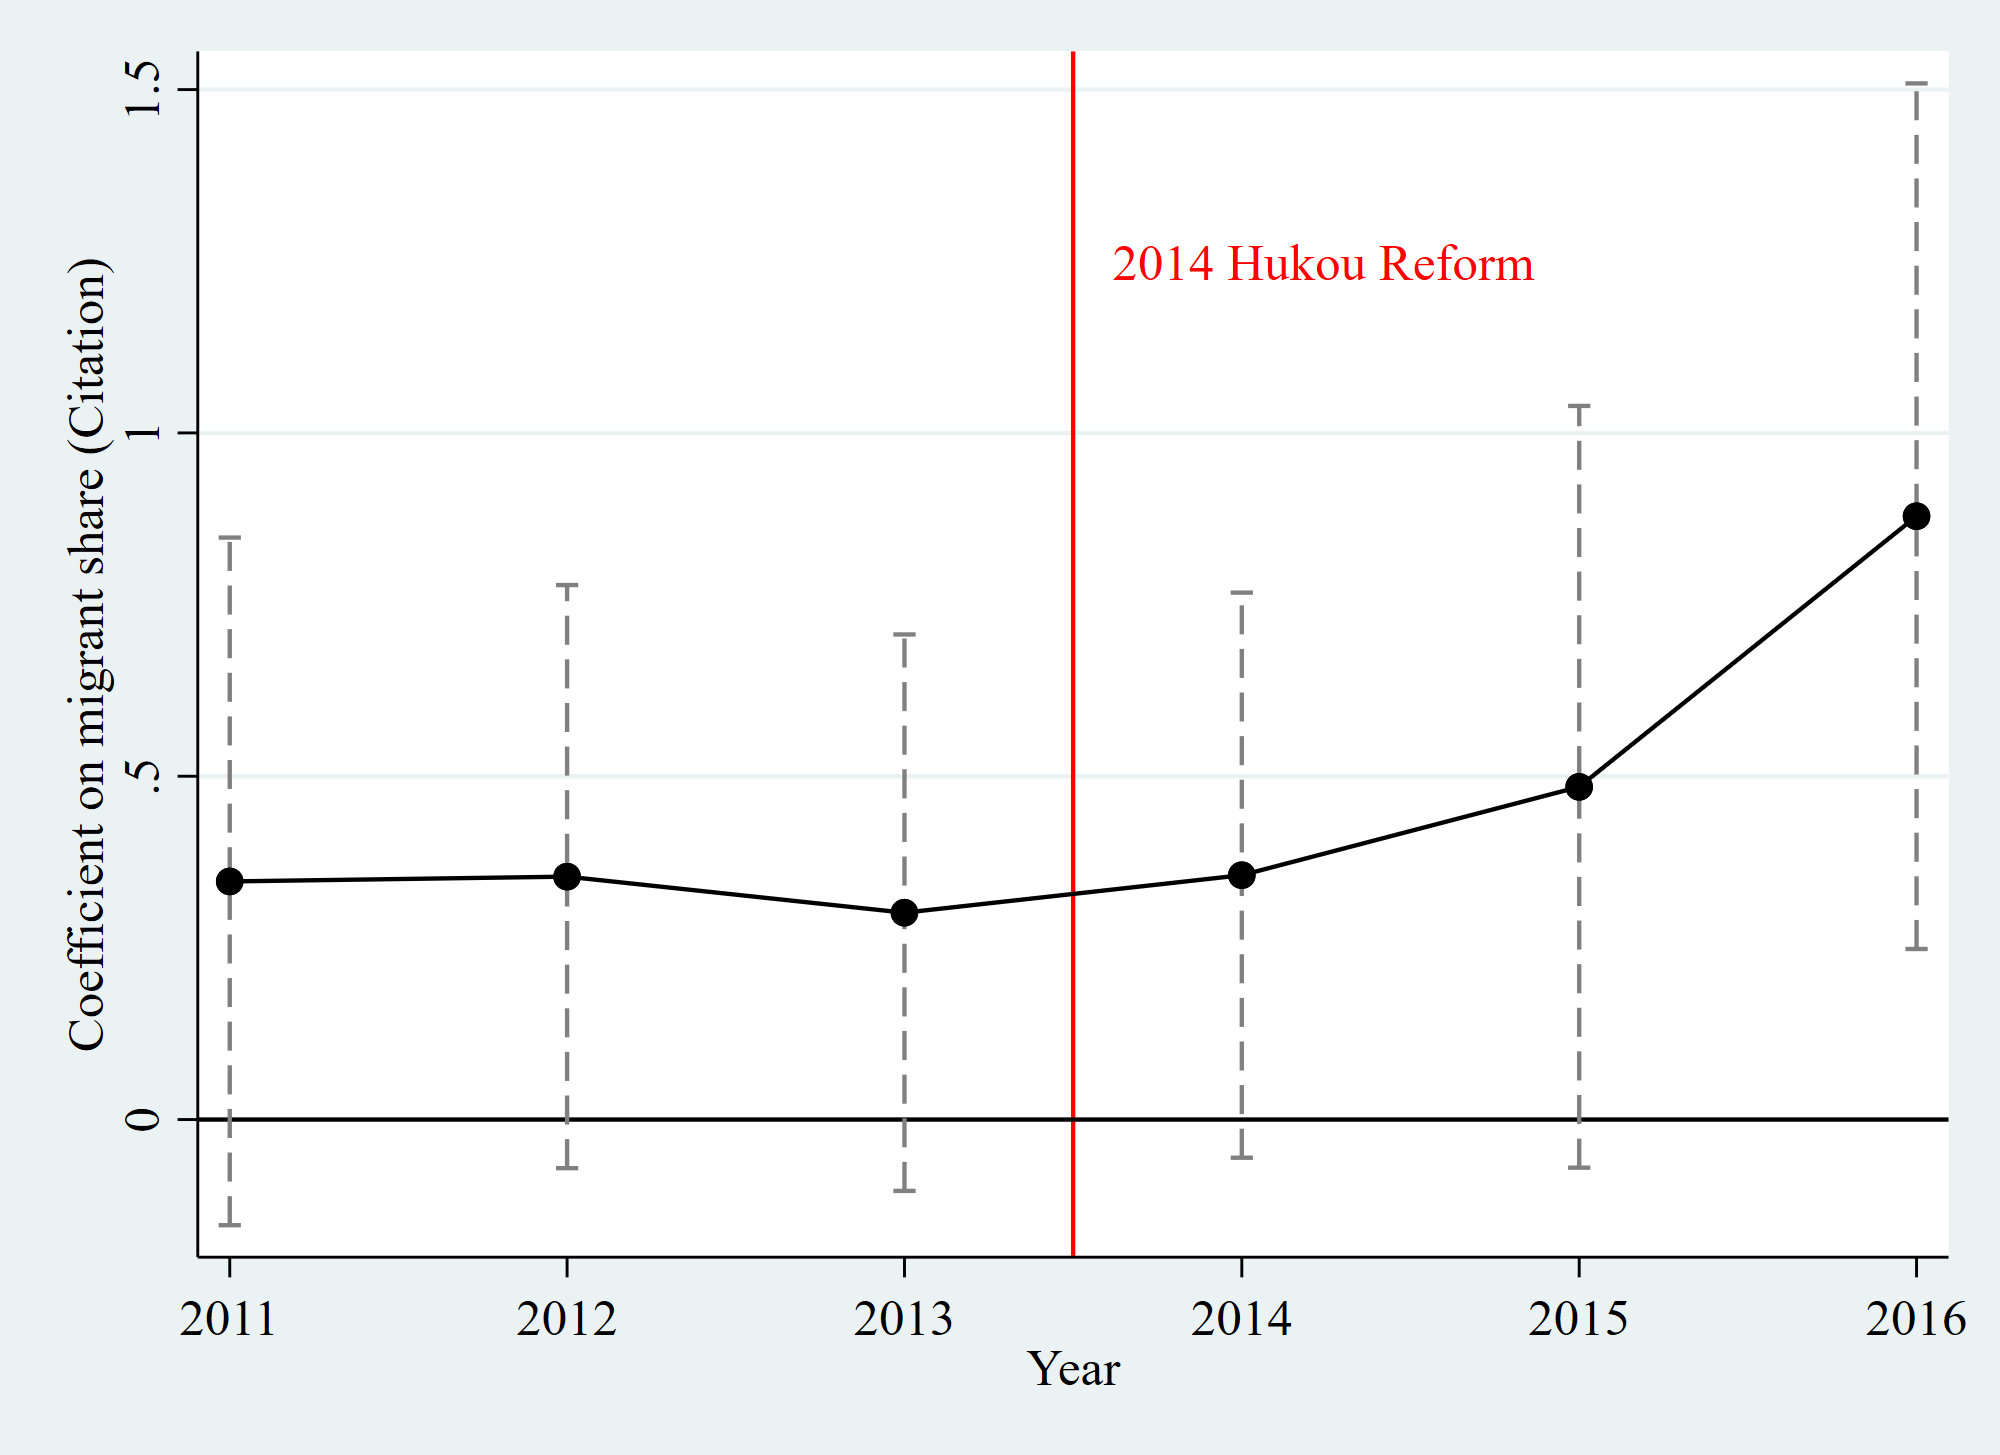
\includegraphics[width=.6\textwidth]{../Analysis/output/pre_trend_iv.png}
  \caption{Effect of Fraction of Immigrants on Knowledge Inflow in Yearly Regression}
  \label{fig:pre_trend}
\end{figure}


%\begin{table}[h]
%  \centering 
%  \resizebox{\textwidth}{!}{
%    \input{../Analysis/output/pre_trend.tex}
%  }
%  \caption{Test exogeneity assumption: pre-trends \vspace{1ex} \\ 
%  {\footnotesize \emph{Notes.} 
% \\ $^{***}$: $p < 0.01$, $^{**}$: $p < 0.05$, $^{*}$: $p < 0.1$.}}
%\end{table}

Figure \ref{fig:pre_trend} plots year-specific 2SLS coefficients from interacting the migrant share with year dummies (city and year FE retained). Points before the 2014 hukou reform (vertical red line) locate around zero and are statistically insignificant, indicating no differential pre-trend in knowledge inflows across cities with higher predicted migrant growth. The effect begins to rise in 2014, becomes visibly larger in 2015, and peaks in 2016. The effect in 2016 is significant positive. This pattern consistent with a short implementation lag, as discussed in Section \ref{sec:high_skill}. Migrants arrive first but do not generate citations immediately, citations follow as patents are granted. Confidence intervals widen in the early years, reflecting fewer observations and lower variation, but the post-reform jump is both economically and statistically meaningful.

\subsection{Shock-level Balance Test}

Broadly, these variables reflect the structure of inflow of immigrants across cities. If the shift are as-good-as-randomly assigned to cities within periods, I expect them to not predict these predetermined variables.

\begin{table}[h]
 \centering 
 \resizebox{\textwidth}{!}{\begin{tabular}{lcccccc} \hline
 & (1) & (2) & (3) & (4) & (5) & (6) \\
VARIABLES & Initial share & Predicted population & Population density & GDP per capita & Industrial added value/GDP & Student ratio \\ \hline
 &  &  &  &  &  &  \\
Shift & -6.40e-10 & 0.000521** & 1.44e-08 & -6.43e-06 & 1.40e-10** & 0 \\
 & (4.62e-10) & (0.000219) & (5.92e-08) & (1.75e-05) & (6.27e-11) & (0) \\
 &  &  &  &  &  &  \\
Number of Cities & 271 & 266 & 268 & 269 & 269 & 268 \\
 $ R^2$ & 0.425 & 0.999 & 0.995 & 0.956 & 0.955 & 0.819 \\ \hline
\end{tabular}
}
 \caption{City covariates balance test \vspace{1ex} \\ 
 {\footnotesize \emph{Notes.} $^{***}$: $p < 0.01$, $^{**}$: $p < 0.05$, $^{*}$: $p < 0.1$.}}
\label{tab:shock_balance1}
\end{table}
\begin{table}[h]
 \centering 
 \resizebox{\textwidth}{!}{
   \begin{tabular}{lcccc} \hline
 & (1) & (2) & (3) & (4) \\
VARIABLES & Average education years & Rural hukou ratio & Male share & Average age \\ \hline
 &  &  &  &  \\
Shift & -8.94e-08*** & 5.46e-09 & 6.27e-09 & 2.28e-07** \\
 & (9.93e-09) & (5.08e-09) & (5.45e-09) & (1.13e-07) \\
 &  &  &  &  \\
Number of Origin-Destination & 3332 & 2895 & 2895 & 2895 \\
 $ R^2$ & 0.443 & 0.574 & 0.312 & 0.489 \\ \hline
\end{tabular}

 }
 \caption{Migrants flow covariates balance test \vspace{1ex} \\ 
 {\footnotesize \emph{Notes.} $^{***}$: $p < 0.01$, $^{**}$: $p < 0.05$, $^{*}$: $p < 0.1$.}}
\label{tab:shock_balance2}
\end{table}

The results in Table \ref{tab:shock_balance1} show that The shift is uncorrelated with initial migrant share, population density, GDP per capita, and the student ratio (coefficients statistically indistinguishable from zero).
Two coefficients reach conventional significance—predicted population and industrial value-added/GDP—but their magnitudes are vanishingly small relative to the scale of the variables. 
Table \ref{tab:shock_balance2} shows that the shift does not predict the rural-hukou share or the male share of migrant inflows. Average education years loads negatively and average age positively but again the coefficients are minute in magnitude. Given multiple outcomes and the very small effect sizes, these isolated rejections are consistent with chance findings rather than systematic imbalance.

Across both tables, the pattern is that exposure-weighted origin shocks exhibit no substantive correlation with predetermined city characteristics or migrant composition. This supports the key SSIV requirement that shocks are orthogonal to observables that might confound the second stage.

\subsection{Alternative Instrument}

\begin{table}[htbp!]
  \centering 
  \resizebox{\textwidth}{!}{
  \begin{tabular}{lccc} \hline
 & (1) & (2) & (3) \\
VARIABLES & ln citation (Baseline) & ln citation (Transportation) & ln citation (Weather) \\ \hline
 &  &  &  \\
Fr. immigrants & 0.657** & 3.130** & -3.573** \\
 & (0.308) & (1.398) & (1.571) \\
 &  &  &  \\
City FE & Yes & Yes & Yes \\
Time FE & Yes & Yes & Yes \\
~ & ~ & ~ & ~ \\
Kleibergen–Paap F-stat & 1408.85 & 10.42 & 11.63 \\
Number of Observations & 11930 & 11961 & 11961 \\
Number of Cities & 265 & 268 & 268 \\
 $ R^2$ & 0.003 & -0.007 & -0.053 \\ \hline
\end{tabular}
}
  \caption{Alternative Instrument \vspace{1ex} \\ 
  {\footnotesize \emph{Notes.} The columns (1)-(3) are baseline instrument, transport shocks and weather shocks, respectively. Standard errors clustered by city.
 \\ $^{***}$: $p < 0.01$, $^{**}$: $p < 0.05$, $^{*}$: $p < 0.1$.}}
 \label{tab:alternative}
\end{table}

A central concern in shift-share designs is that the instrument may conflate genuine migrant-driven shocks with omitted demand or supply factors correlated across cities. To address this, I implement a set of alternative instruments. The alternative instruments below are targeted stress tests for distinct violations of the baseline assumptions; they are not substitutes but diagnostic checks of identification.

Table \ref{tab:alternative} evaluates two placebo test using alternative shift-share instruments that replace the province-year shift $g_{ot}$ with two plausibly exogenous origin-side shocks including transport-network expansion and weather disasters. The share component (2010 migrant distribution across cities) remains unchanged.

The benchmark IV from in column 1 yields a significant positive effect with strong first stage.

Column 2 uses transportation construction as instrument: 

\begin{equation*}
  Z_{transport}= \frac{1}{\hat{Pop}_{dt}}\sum_{o \neq \text{}(d)}  s_{od}^{2010}\times \text{Density}_{ot}
\end{equation*}

where $\text{Density}_{ot}$ is the kilometer of newly opened rail or expressway lines per square kilometer in origin province $o$ in year $t$. The coefficient rises to 3.1 and remains significant at 5\%, indicating that emigration triggered by infrastructure construction are even more strongly associated with knowledge inflows. The first-stage F-statistic is above the threshold but far weaker than in the baseline. This finding is consistent with \cite{douPainGainEffects2024} who find that transport infrastructure expansion induces the population mobility. 

The column 3 use weather shocks as instrument: 
\begin{equation*}
  Z_{weather}= \frac{1}{\hat{Pop}_{dt}}\sum_{o \neq \text{}(d)}  s_{od}^{2010}\times \text{Affected}_{ot}
\end{equation*}
, where $\text{Affected}_{ot}$ is the share of cropland hit by natural disasters. The coefficient flips sign to -3.5 and is significant, aligning with \cite{imbertMigrantsFirmsEvidence2022} who find weather-driven migration reduces firm-level innovation in China. Conceptually, weather shocks primarily induce rural-to-urban moves, so the associated migrants may lack the human capital or networks that foster patent-based knowledge flows.

The transport-based IV corroborates the main finding, while the weather-based IV highlights a qualitatively different mechanism. Crucially, neither alternative instrument overturns the evidence that migrant inflows matter for knowledge inflow. However, the weaker first-stage strength cautions against relying solely on these shocks. I therefore treat them as auxiliary robustness checks rather than primary identification.

Across designs, the baseline SSIV remains the workhorse. The transport IV primarily probes shift endogeneity using origin-side costs; the weather IV probes destination pull and treatment-composition. Concordant signs with attenuated precision support the interpretation that the main results are not driven by destination demand and that effects are larger when inflows are more skill-intensive.




\section{Conclusion} \label{sec:conclusion}

This dissertation studies whether internal migration facilitates the diffusion of technological knowledge across Chinese cities. Using city--year flows of backward patent citations as the outcome and a shift-share instrument to address endogeneity in migrant inflows, the analysis links migrants origin provinces to directional knowledge inflows at destinations. The identification strategy targets concerns about omitted variables and reverse causality, by leveraging origin-specific migration shocks interacted with historical migrant shares in a leave-out design.

Four sets of findings emerge. First, cities that experience higher migrant inflows see higher knowledge inflows. In IV specifications, a one-percentage-point increase in the migrant share is associated with a 0.65\% increase in backward citations. The IV estimates are smaller than OLS, consistent with positive selection of migrants into already innovative locations. Second, composition matters: high-skilled migrants are associated with larger knowledge inflows than the average migrant, with point estimates around five times the baseline IV effect. By contrast, effects for very recent arrivals are positive in parsimonious models but attenuate to statistical insignificance once full controls are included, suggesting contributions materialise with some lag or are mediated by compositional differences. Third, the effect is concentrated in invention patents rather than utility models, indicating that migration is more closely linked to the diffusion of higher-novelty knowledge. Estimates for external and self-citations is significant positive, implying that immigrants can both bring knowledge indirectly and direclty. Finally, there is significant regional heterogeneity. Estimated effects are small on the eastern coast and considerably larger inland. In particular, central and western cities exhibit higher elasticities, consistent with knowledge flowing from more advanced to less advanced regions. The very large central-region coefficient should be interpreted with caution and viewed in light of sample composition, the LATE nature of IV estimates, and potential sensitivity to specification.

The contribution of this study is threefold. It provides evidence on the role of internal migration—rather than international flows—in shaping innovation; it uses directional patent-citation links to measure within-country knowledge transmission at the city level; and it documents heterogeneity by migrant composition, region, and patent type. 

According to the results, there are several policy implications. First, easing settlement restrictions for educated migrants is likely to yield measurable innovation pay-offs, particularly for inland cities that currently lag on R\&D. Second, scholarship or housing programmes that attract university-educated workers may be more cost-effective than broad relocation subsidies. Additionally, the transport-shock instrument suggests that building connectivity in origin provinces not only pushes out labour but also transmits knowledge to receiving cities.

Finally, the study has some limitations. First, citations miss informal knowledge flows and non-patented innovation. Matching migrants to scientific publications, trade secrets, or venture-capital networks would paint a fuller picture. The study only focuses on the inflow aspect of knowledge inflow, and does not consider the outflow aspect. The outflow of knowledge may also have an impact on the knowledge inflow in the city. Second, instrument validity in the long run. While the first stage is strong, province-level shocks might still correlate with unobserved demand trends. Third, data limitations. This panel ends in 2016. Extending the analysis through the post-COVID era would capture recent shifts in internal mobility and digital collaboration. This data also lacks micro mechanisms. Firm or inventor level data could disentangle whether migrants bring ideas directly, act as bridge builders, or simply raise competitive pressure that spurs local firms to learn.




\clearpage
\addcontentsline{toc}{section}{References}
\bibliographystyle{agsm}
\bibliography{Library.bib}



\clearpage

\section*{Appendix} \label{sec:appendixa}
\addcontentsline{toc}{section}{Appendix}
\begin{figure}[h]
  \centering
  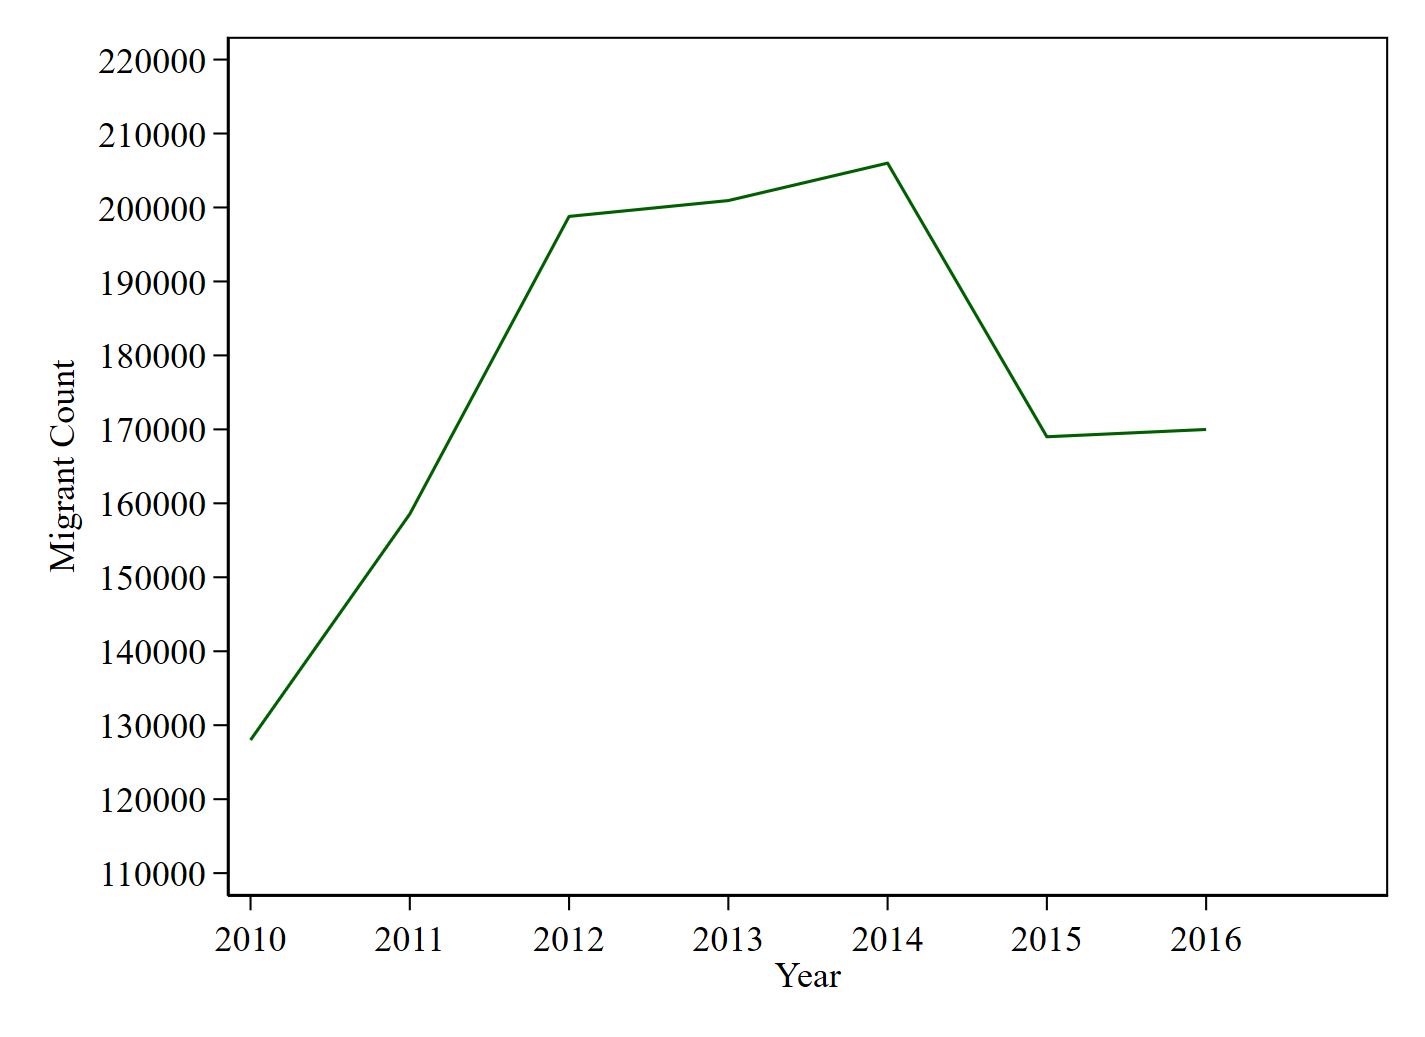
\includegraphics[width=.6\textwidth]{../Analysis/output/sample_size.png}
  \caption{Sample Size of Each Year, 2010 - 2016}
\end{figure}


\begin{figure}[h]
  \centering
  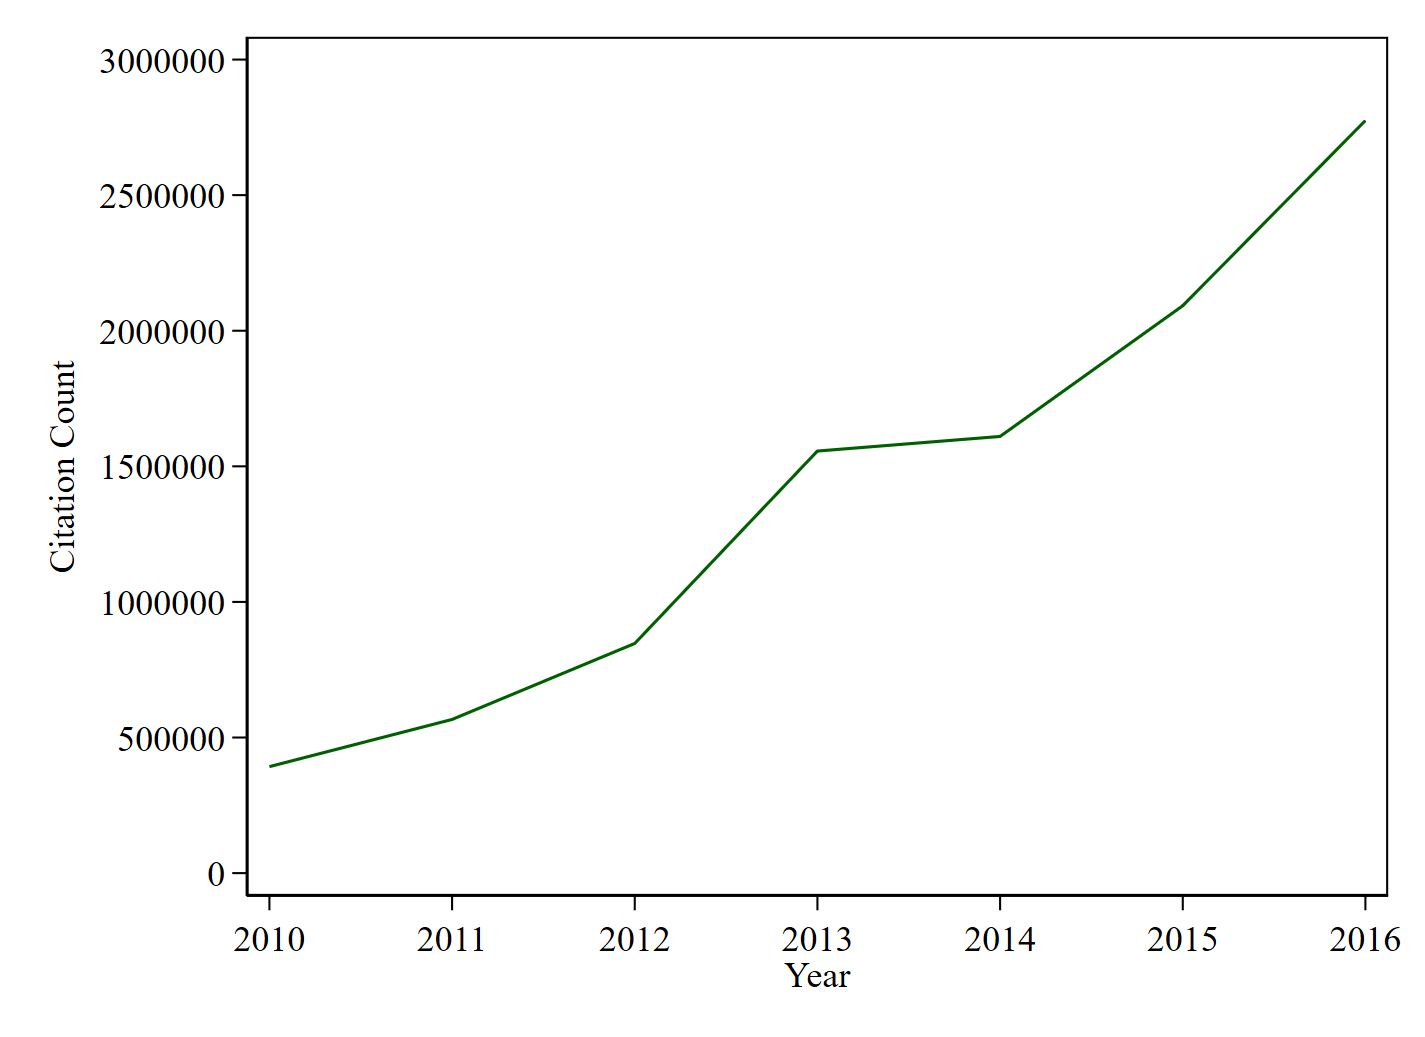
\includegraphics[width=.6\textwidth]{../Analysis/output/Citation_over_time.png}
  \caption{Annual Citation Counts, 2010 - 2016}
\end{figure}

% 2011-2016
\begin{figure}[!htbp]
    \centering
    % 2011
    \begin{subfigure}{0.45\textwidth}
        \centering
        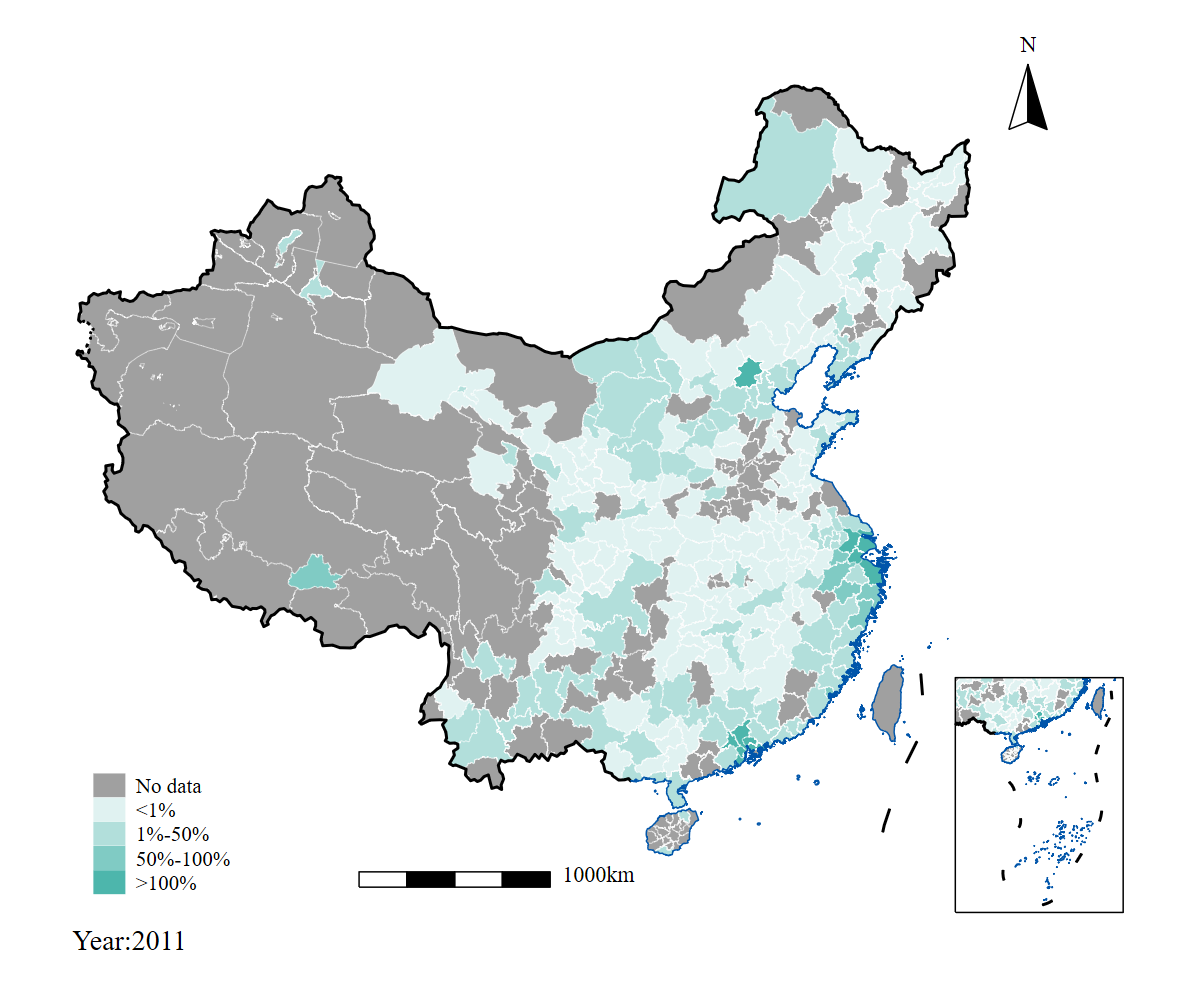
\includegraphics[width=\textwidth]{../Analysis/output/figure_immgrants_share_2011.png}
        \label{fig:2011}
    \end{subfigure}
    \hfill
    % 2012
    \begin{subfigure}{0.45\textwidth}
        \centering
        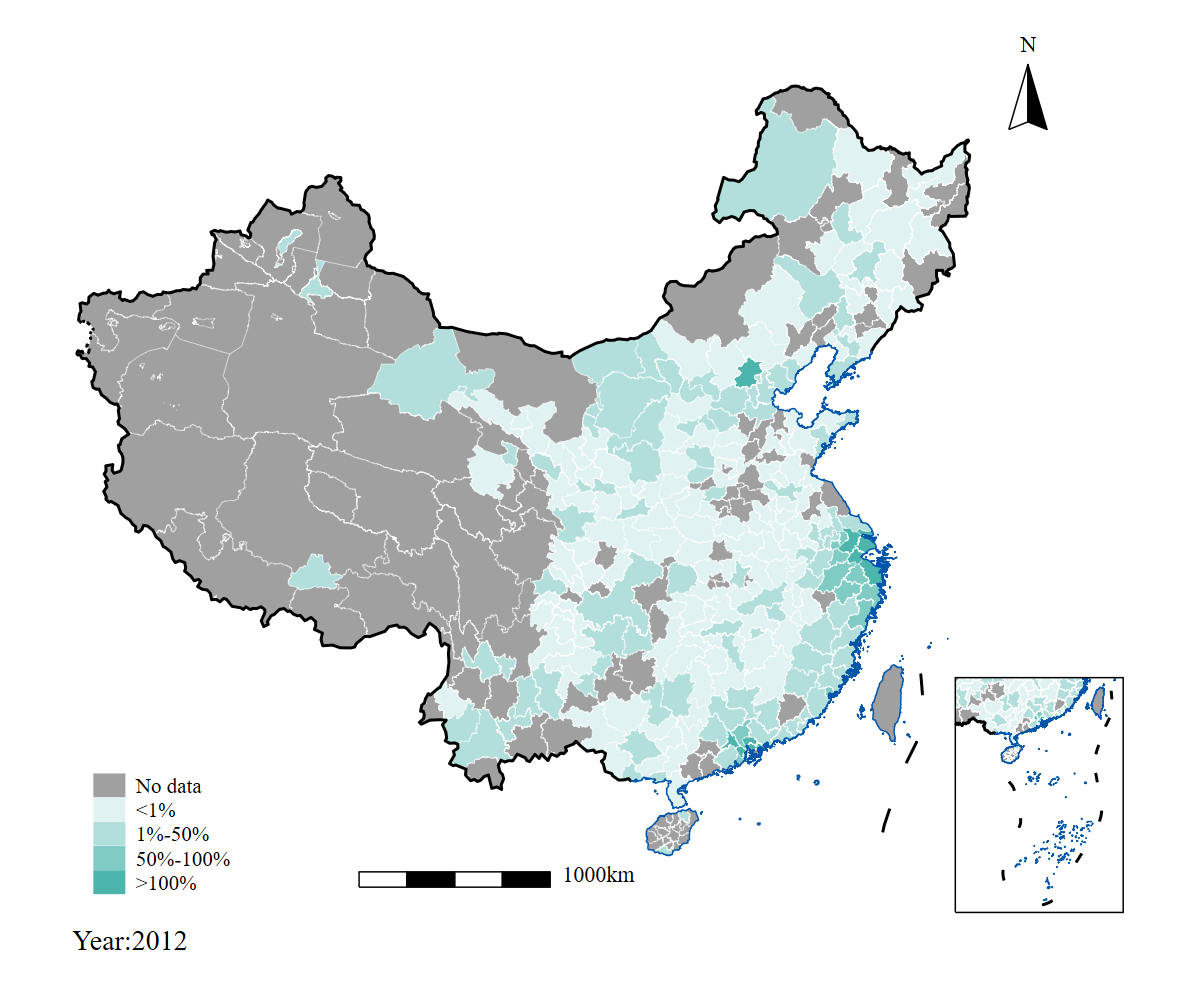
\includegraphics[width=\textwidth]{../Analysis/output/figure_immgrants_share_2012.png}
        \label{fig:2012}
    \end{subfigure}
    \hfill
    % 2013
    \begin{subfigure}{0.45\textwidth}
        \centering
        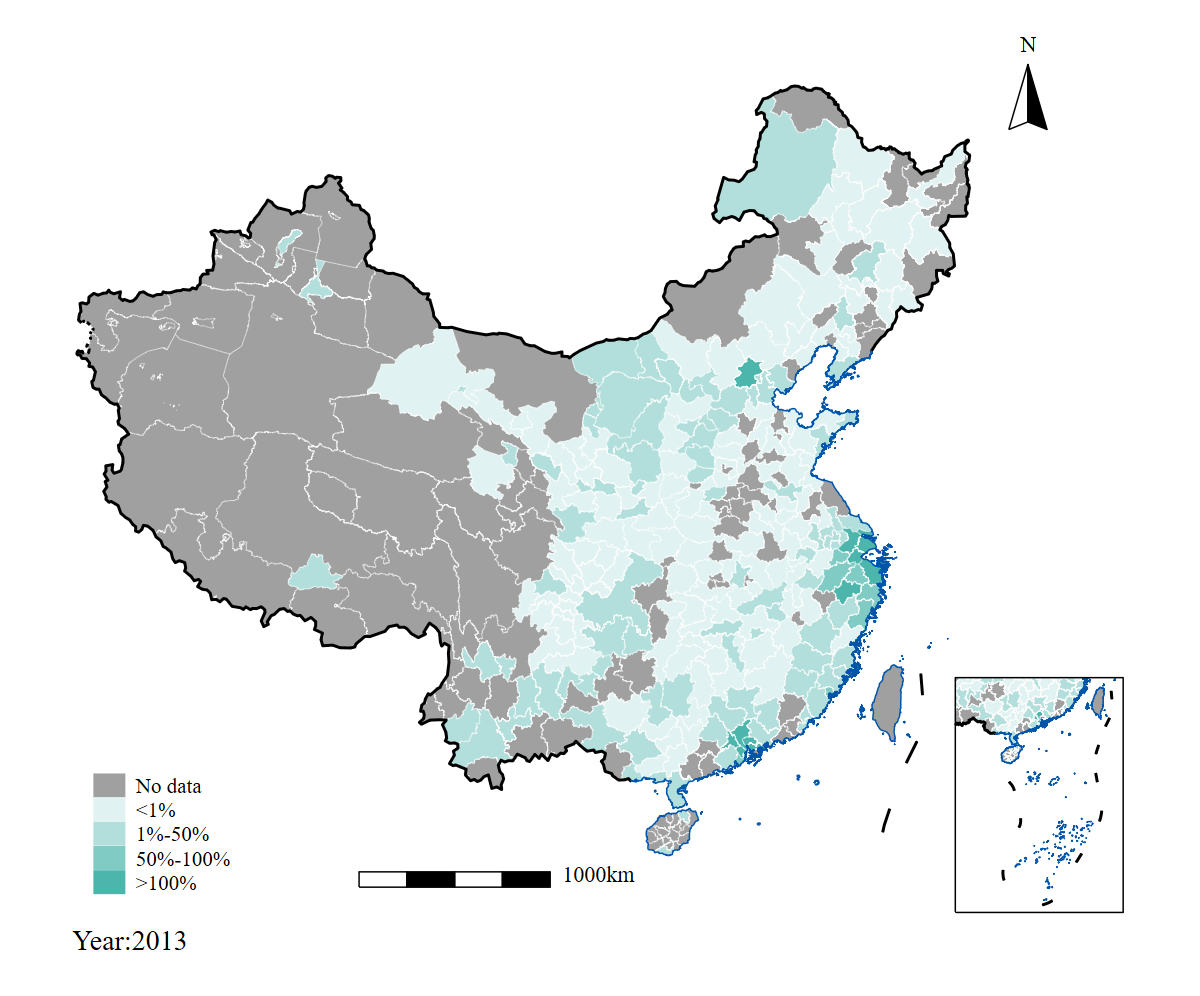
\includegraphics[width=\textwidth]{../Analysis/output/figure_immgrants_share_2013.png}
        \label{fig:2013}
    \end{subfigure}
    \hfill
    \begin{subfigure}{0.45\textwidth}
        \centering
        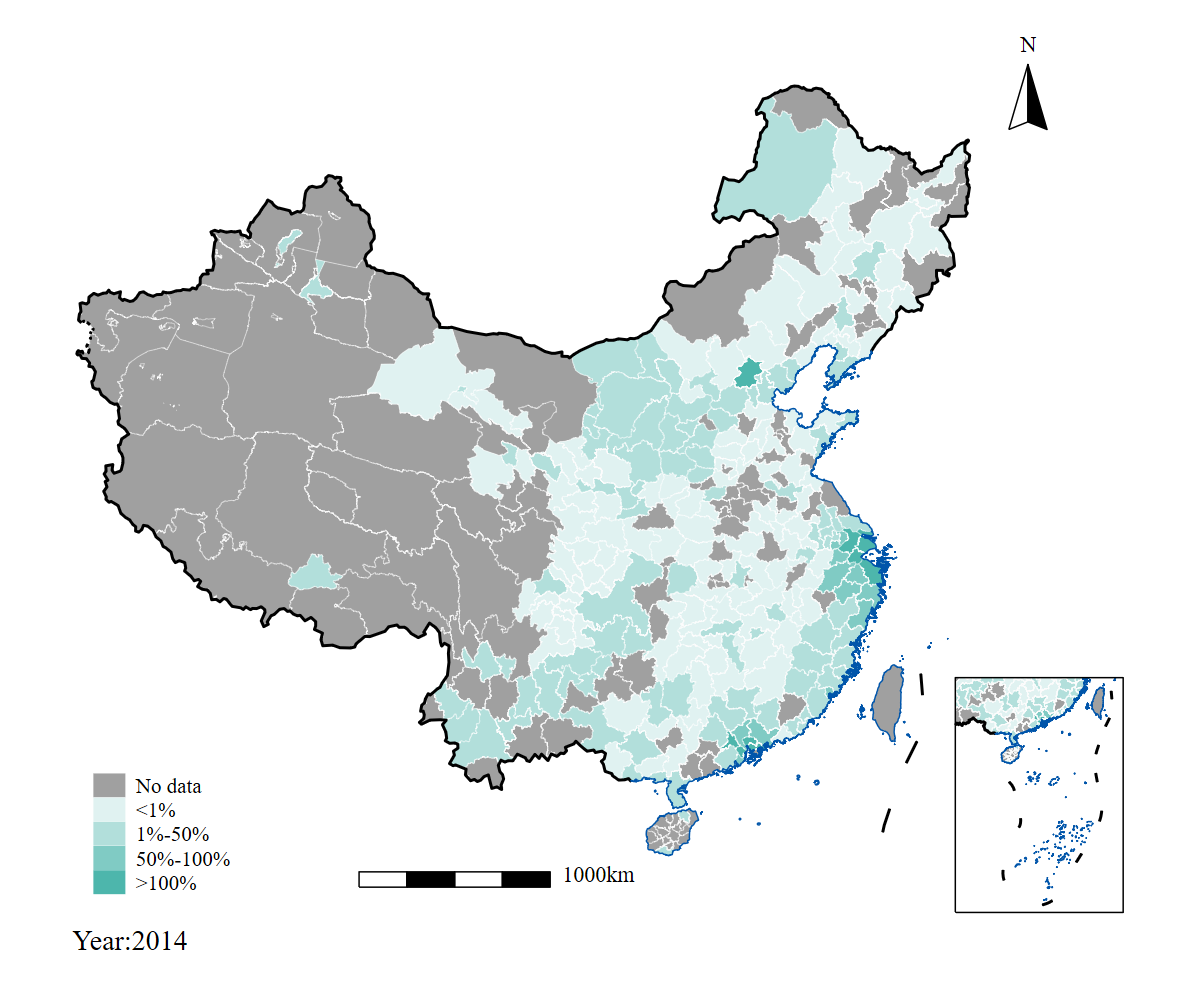
\includegraphics[width=\textwidth]{../Analysis/output/figure_immgrants_share_2014.png}
        \label{fig:2014}
    \end{subfigure}
    \hfill
    \begin{subfigure}{0.45\textwidth}
        \centering
        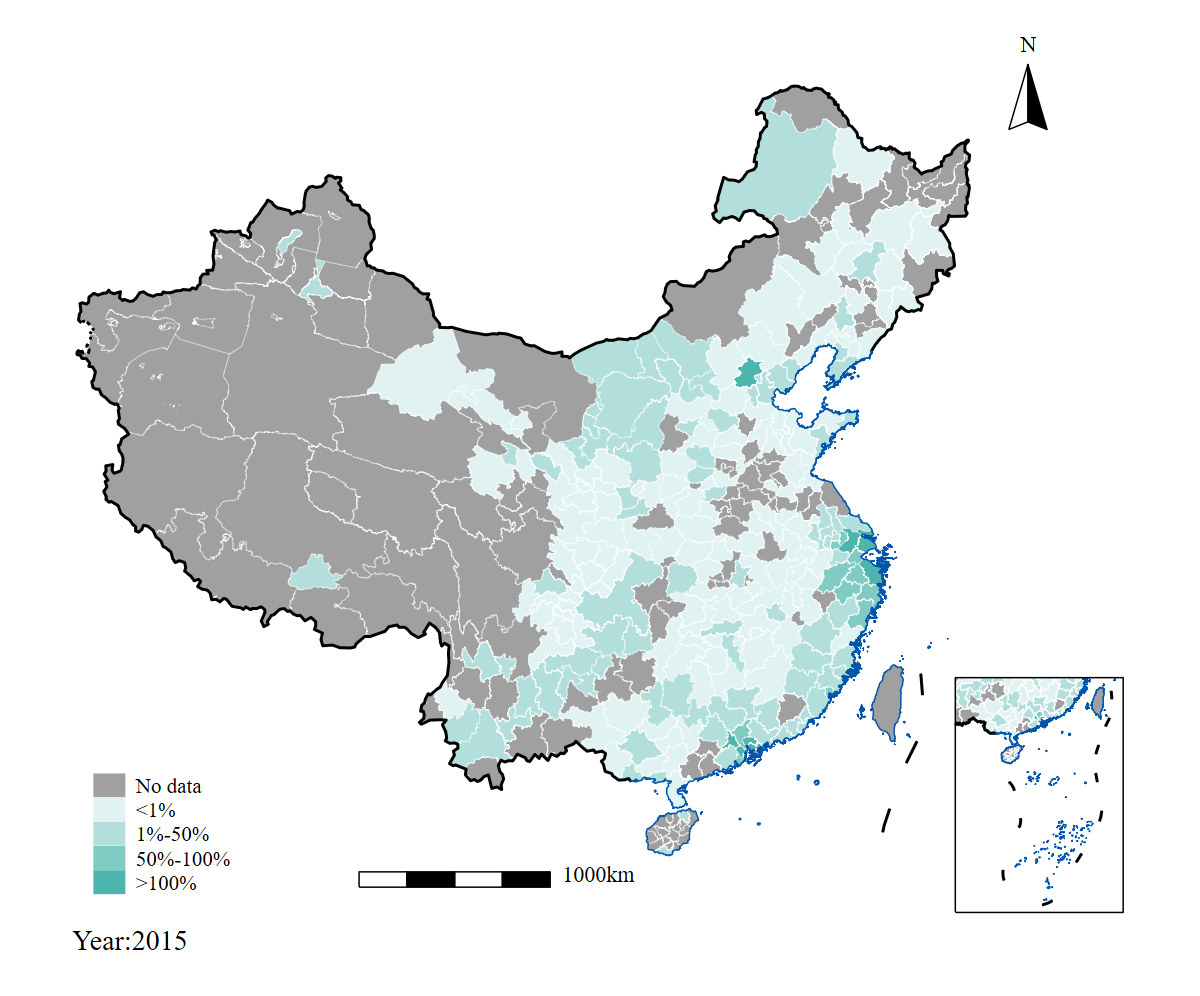
\includegraphics[width=\textwidth]{../Analysis/output/figure_immgrants_share_2015.png}
        \label{fig:2015}
    \end{subfigure}
    \hfill
    \begin{subfigure}{0.45\textwidth}
        \centering
        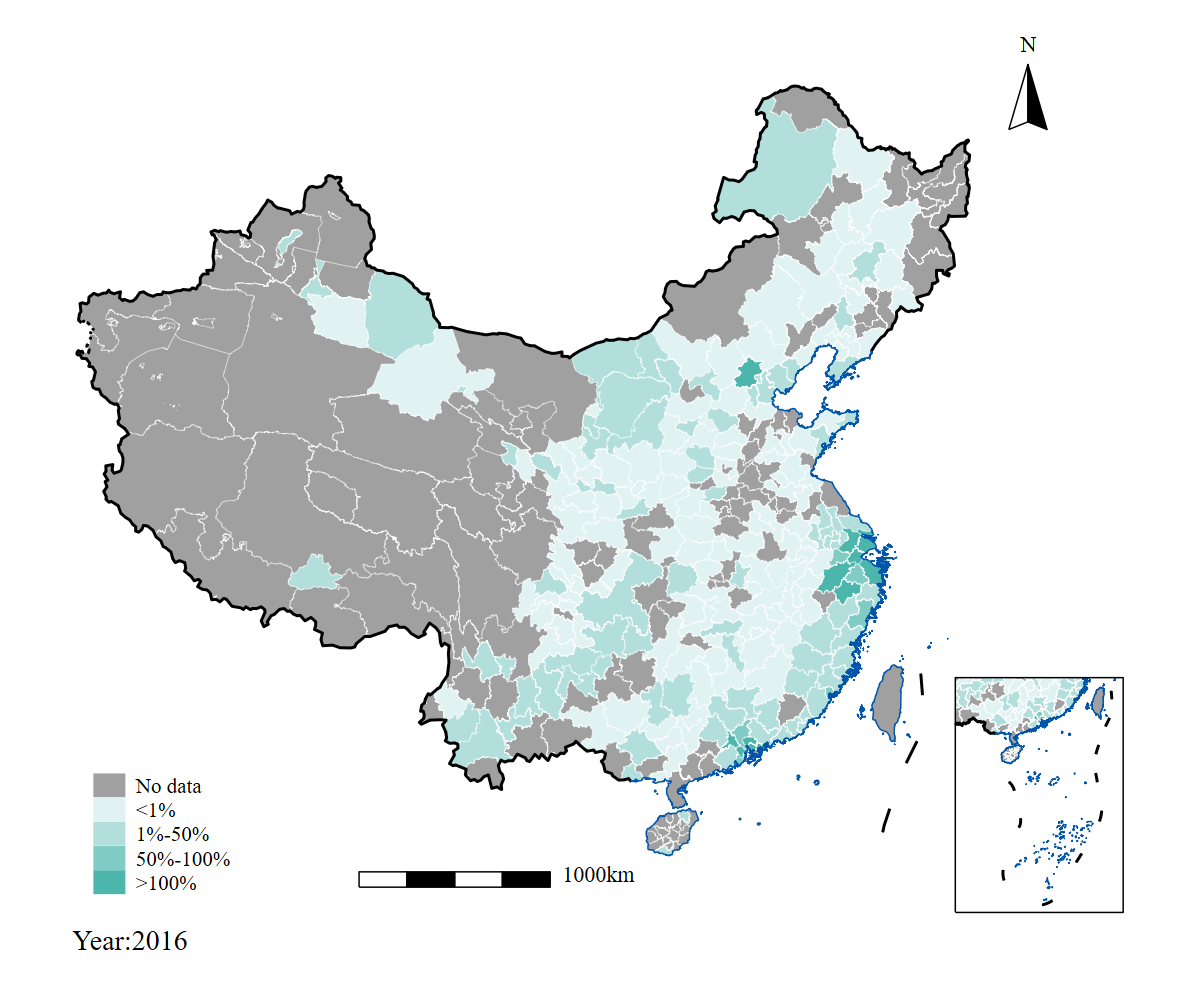
\includegraphics[width=\textwidth]{../Analysis/output/figure_immgrants_share_2016.png}
        \label{fig:2016}
    \end{subfigure}
    \caption{Fraction of \emph{Aggregated} Immigrants in Cities, 2011-2016 \vspace{1ex} \\ 
    {\footnotesize \emph{Notes.} The metric plotted is each city's fraction of the \emph{sum of immigrants whose province of origin differs from the destination city} relative to that city's total resident population in the given year, which is an aggregate of \emph{Fr. immigrants} in table \ref{tab:summary}. Grey areas indicate cities with no available data.}}
   \label{fig:combined_figure_summary}
\end{figure}


\end{document}